\documentclass[conference]{IEEEtran}

\title{\tool{}: Scalable Analysis of \\ Weakly-Hard Constraints}
\author{Nils Vreman$^1$, Richard Pates$^1$, Martina Maggio$^{2,1}$\\
$^1$Lund University, Sweden\\
$^2$Saarland University, Germany
\thanks{The authors are members of the ELLIIT Strategic Research Area at Lund University. 
This project has received funding from the European Union's Horizon 2020 research and innovation programme under grant agreement Number 871259 (ADMORPH project). 
This publication reflects only the authors' view and the European Commission is not responsible for any use that may be made of the information it contains.}}

%%%%%%%%%%%%%%%%%%%%%%%%%%%%%%%%%%%%%%%%%%%%%%%%%%%%%%%%%%%%%%%%%%%%%%%%%%%%%%%%
% In this file, only packages are allowed. These packages should be explained to
% greatest possible extent.
%%%%%%%%%%%%%%%%%%%%%%%%%%%%%%%%%%%%%%%%%%%%%%%%%%%%%%%%%%%%%%%%%%%%%%%%%%%%%%%%

% Document encodings
\usepackage[english]{babel}
\usepackage[utf8]{inputenc}
\usepackage[T1]{fontenc} % This can slightly change font appearance
\usepackage{xcolor} 

% Beamer theme
\usepackage{style/beamertheme} % Needes XeLaTeX

% Math related
\usepackage{amsmath, amssymb, amsthm, mathtools}
\usepackage{xfrac} %for nice inline fractions

% Char. related 
\usepackage{microtype}

% Bibliography related
\usepackage[backend=biber, style=authoryear]{biblatex}
\addbibresource{defence.bib}
\renewcommand*{\nameyeardelim}{\addcomma\space}
\AtBeginBibliography{\scriptsize}

%\usepackage{multirow} % For multirow tables
%\usepackage{colortbl} % For coloured tables

% Colordefinitions
\definecolor{misscolour}{RGB}{255, 0, 0}
\definecolor{lqrcolour}{RGB}{0,28,255}
\definecolor{lqrnomcolour}{RGB}{0,28,255}
\definecolor{lqgcolour}{RGB}{0,139,0}
\definecolor{lqgnomcolour}{RGB}{0,139,0}
\definecolor{adacolour}{RGB}{239,133,16}

\definecolor{baselinecolor}{rgb}{0.9, 0.78, 0.07}
\definecolor{markcolor}{rgb}{0.6, 0.64, 0.69}

\definecolor{hicolour}{RGB}{50, 50, 255}

% Tikz packages and related
\usepackage{tikz} 
\usepackage{pgfplots, pgfplotstable} 
\usepackage{fontawesome5} 

% Tikz Libraries
\usepgfplotslibrary{external}
    \tikzexternalize[prefix=tikz/]
    \tikzset{external/system call={lualatex \tikzexternalcheckshellescape
        -halt-on-error -interaction=batchmode -jobname "\image" "\texsource"}
    } % to let pdflatex work

\usepgfplotslibrary{groupplots}
\usepgfplotslibrary{fillbetween}
\pgfplotsset{colormap/viridis}
\pgfplotsset{compat=newest}
\usetikzlibrary{decorations.markings}
\usetikzlibrary{shapes}
\usetikzlibrary{backgrounds}
\usetikzlibrary{fit}

\usetikzlibrary{calc}
\usetikzlibrary{arrows}
\usetikzlibrary{arrows.meta}
\usetikzlibrary{patterns, patterns.meta}
\usetikzlibrary{shapes.misc}
%\pgfplotsset{compat=1.16}

%\usepgfplotslibrary{fillbetween}
\usetikzlibrary{positioning}
%\usepackage{makecell} 

%%% RTAS22B
\tikzset{Dom Node/.style={draw,
                        thick,
                        circle,
                        inner sep=0pt,
                        minimum size=12mm}%
}%
\tikzset{
    old inner xsep/.estore in=\oldinnerxsep,
    old inner ysep/.estore in=\oldinnerysep,
    Init Node/.style 2 args={draw,
                    thick,
                    circle,
                    minimum size=12mm,
                    old inner xsep=\pgfkeysvalueof{/pgf/inner xsep},
                    old inner ysep=\pgfkeysvalueof{/pgf/inner ysep},
                    /pgf/inner xsep=\oldinnerxsep+#1,
                    /pgf/inner ysep=\oldinnerysep+#1,
                    alias=sourcenode,
                    append after command={
                    let     \p1 = (sourcenode.center),
                            \p2 = (sourcenode.east),
                            \n1 = {\x2-\x1-#1-0.5*\pgflinewidth}
                    in
                        node [inner sep=0pt, draw, circle, minimum width=2*\n1,at=(\p1),#2] {}
                    }
    },
    Init Node/.default={2pt}{black}%
}%

%%% Comparison figure related
\def\xstart{1}
\def\xend{10} % change according to how many plots you have

% this is the list of styles
% define as many colours as the number of lines
% you could also change the marker etc
\pgfplotscreateplotcyclelist{blue10}{
    {blue!95!black, mark=*, mark size=2pt,mark options={fill=white}},
    {blue!85!black, mark=*, mark size=2pt},
    {blue!75!black, mark=*, mark size=2pt},
    {blue!65!black, mark=*, mark size=2pt},
    {blue!55!black, mark=*, mark size=2pt},
    {blue!45!black, mark=*, mark size=2pt},
    {blue!35!black, mark=*, mark size=2pt},
    {blue!25!black, mark=*, mark size=2pt},
    {blue!15!black, mark=*, mark size=2pt},
    {blue! 5!black, mark=*, mark size=2pt},
}

% argument #1: any options
\makeatletter
\newenvironment{customlegend}[1][]{%
    \begingroup
    % inits/clears the lists (which might be populated from previous
    % axes):
    \pgfplots@init@cleared@structures
    \pgfplotsset{#1}%
}{%
    % draws the legend:
    \pgfplots@createlegend
    \endgroup
}%

% makes \addlegendimage available (typically only available within an
% axis environment):
\def\addlegendimage{\pgfplots@addlegendimage}
\makeatother

%%% ECRTS 
\tikzset{cross/.style={%
    cross out,
    draw,
    minimum size=2*(#1-\pgflinewidth),
    inner sep=0pt, outer sep=0pt}}

\makeatletter
\pgfplotsset{
    every axis plot/.append style =
    {mark=none, mark options={fill=white}},
    mark max/.style={
        scatter/@pre marker code/.code={%
            \ifx\pgfplotspointmeta\pgfplots@metamax
                \def\markopts{}%
                \node [anchor=south, xshift=1mm, yshift=-0.4mm] { \pgfmathprintnumber[precision=1, fixed zerofill]{\pgfplotspointmeta} };
            \else
                \def\markopts{mark=none}
            \fi
                \expandafter\scope\expandafter[\markopts]
        },%
        scatter/@post marker code/.code={ \endscope },
        scatter
    }
}
% Style to select only points from #1 to #2 (inclusive)
\pgfplotsset{select coords between index/.style 2 args={
    x filter/.code={
        \ifnum\coordindex<#1\def\pgfmathresult{}\fi
        \ifnum\coordindex>#2\def\pgfmathresult{}\fi
    }
}}
\makeatother

\newcommand{\findmax}[1]{
    \pgfmathsetmacro\buffer{0.0}
    \pgfplotstableforeachcolumnelement{#1}\of\extdata\as\cellValue{%
        \pgfmathsetmacro{\buffer}{max(\buffer,\cellValue)}}
}
\newcommand*{\ReadOutElement}[4]{%
    \pgfplotstablegetelem{#2}{[index]#3}\of{#1}%
    \let#4\pgfplotsretval
}

%%%%%%%%%%%%%%%%%%%%%%%%%%%%%%%%%%%%%%%%%%%%%%%%%%%%%%%%%%%%%%%%%%%%%%%%%%%%%%%%
% In this file, only commands are allowed. These commands should be explained to
% greatest possible extent.
%%%%%%%%%%%%%%%%%%%%%%%%%%%%%%%%%%%%%%%%%%%%%%%%%%%%%%%%%%%%%%%%%%%%%%%%%%%%%%%%

%%% Blame commands
\newcommand{\pointout}[1]{\color{red}#1\color{black}} 

% Simplifying commands
\newcommand{\tool}{\texttt{\textbf{WeaklyHard.jl}}}
\newcommand{\toolL}{\texttt{\textbf{WHRTgraph}}}

% Maths general
\newcommand{\funof}[1]{\left( #1 \right)}
\newcommand{\abs}[1]{\left|#1\right|}
\newcommand{\norm}[1]{\left\lVert#1\right\rVert}
\DeclareMathOperator*{\argmax}{argmax}
\DeclareMathOperator*{\argmin}{argmin}
\newcommand{\nequiv}{\not\equiv}
\newcommand{\ourmod}[1]{\ \mathrm{mod}\ #1}
\newcommand{\tr}[1]{\mathrm{tr}\left(#1\right)} 

% Constraint names
\newcommand{\tAH}{\texttt{\textbf{AnyHit}}}
\newcommand{\tAM}{\texttt{\textbf{AnyMiss}}}
\newcommand{\tRH}{\texttt{\textbf{RowHit}}}
\newcommand{\tRM}{\texttt{\textbf{RowMiss}}}

% Constraints related
\newcommand{\anyhit}[1]{\binom{x_{#1}}{k_{#1}}}
\newcommand{\anymiss}[1]{\overline{\binom{x_{#1}}{k_{#1}}}}
\newcommand{\rowhit}[1]{\genfrac{<}{>}{0pt}{}{x_{#1}}{k_{#1}}}
\newcommand{\rowmiss}[1]{\overline{\genfrac{<}{>}{0pt}{}{x_{#1}}{k_{#1}}}}
\newcommand{\sset}[2]{\mathcal{S}_{#1}\funof{#2}}
\newcommand{\lweak}{\underline{\lambda}}
\newcommand{\lhard}{\overline{\lambda}}

\DeclarePairedDelimiter\ceil{\lceil}{\rceil}
\DeclarePairedDelimiter\floor{\left\lfloor}{\right\rfloor}

% Aliases in general
\newcommand{\strat}{\mathcal{H}} 
\newcommand{\LL}[1]{\mathcal{L}_{#1}} 
\newcommand{\overbar}[1]{\mkern 1.5mu\overline{\mkern-1.5mu#1\mkern-1.5mu}\mkern 1.5mu}

% Automaton related
\newcommand{\GG}[1]{\mathcal{G}_{#1}}                               % Automaton
\newcommand{\VV}[1]{V_{#1}}                                         % Nodes
\newcommand{\EE}[1]{E_{#1}}                                         % Edges
\newcommand*\BitAnd{\mathbin{\&}}
\newcommand*\BitOr{\mathbin{|}}
\newcommand*\ShiftLeft{\ll}
\newcommand*\ShiftRight{\gg}
\newcommand*\BitNeg{\ensuremath{\mathord{\sim}}}

% Figure related
\newcommand{\binsaggregatedhist}[0]{65}


\IEEEoverridecommandlockouts

\begin{document}
%% ARTIFACT EVALUATION STAMP - START
\makeatletter
\def\@artifactstamptop{0.1cm}
\def\@artifactstampright{0.1cm}
\def\@artifactstampwidth{2.5cm}
\let\@aetitle\@maketitle
\def\@maketitle{
\begin{tikzpicture}[remember picture,overlay,shift={(current page.north east)}]%
\node[anchor=north east,xshift=-\@artifactstampright,yshift=-\@artifactstamptop]{\includegraphics[width=\@artifactstampwidth]{badge_rtas_AE}};%
\end{tikzpicture}%
\@aetitle}
\makeatother
%% ARTIFACT EVALUATION STAMP - END


\maketitle

\begin{abstract}
Weakly-hard models have been used to analyse real-time systems subject to patterns of deadline hits and misses. However, the tools that are available in the literature have a set of shortcomings. The analysis they offer is limited to a single weakly-hard constraint and to patterns that specify the number of misses, rather than the number of hits. Furthermore, the scalability of the tools is limited, effectively making it hard to address systems where deadline misses are really sporadic events. In this paper we present \tool{}, a scalable tool to analyse a set of weakly hard constraints belonging to all the four types of weakly hard models. To achieve scalability, we exploit novel dominance relations between weakly-hard constraints, based on deadline hits. We provide experimental evidence of the tool's scalability, compared to the state-of-the-art for a single constraint, a thorough investigation of hit-based weakly-hard constraints, and a sensitivity analysis to constraint set parameters.
\end{abstract}

\begin{IEEEkeywords}
Weakly-Hard Task Model, Deadline Miss
\end{IEEEkeywords}

\section{Introduction}
\label{sec:intro}
Robustness is an essential concern in the design of control systems; they must be able to reliably handle nonlinear effects, unmodeled dynamics and noise, as well as delays in signal transmissions and dropped packets.
A lesser known problem concerns the assessment of robustness to \emph{computational issues} when controllers are implemented as periodic tasks in cheap embedded platforms.
Such tasks are expected to execute with real-time guarantees, i.e., their execution must be completed before a well-defined \emph{deadline}, when the control output must be sent to the actuator.
However, it is common in practice~\cite{akesson2020empirical} that tasks do not always complete within their deadline, causing what is called a \emph{deadline miss}.
This may be caused by delays in computation and memory accesses, transient overloads, bugs and other issues.

A popular model to describe real-time systems allowing deadline misses is the \emph{weakly-hard} model~\cite{Bernat:2001}. 
Weakly-hard tasks feature constraints defining a maximum number of deadlines that can be missed (alternatively, a minimum number to be satisfied) in a given number of consecutive periods.
This model is also the focus of this work.
To analyse the effects on the controlled plant, it is necessary to specify also \emph{what happens when the miss is experienced}, both in terms of changes to the control signal and of actions taken to deal with the failed computation~\cite{Pazzaglia:2019}.
An instance that experiences a deadline miss can be allowed to continue executing until completion (and possibly used later), while in other applications it is stopped and discarded instead.

There is however a mismatch between the guarantees that can be obtained for real-time tasks and platforms~\cite{Ernst:2015,choi2019job}, and the analysis available for \emph{control} tasks under the weakly-hard model.
Fewer works deal with \emph{stability} analysis of weakly-hard real-time control tasks, often targeting specific use-cases. 
For instance, the analysis in~\cite{Maggio:2020} is limited to constraints specifying a maximum number of \emph{consecutive} deadline misses.
The results in \cite{Linsenmayer:2017,linsenmayer2020linear}, obtained for networked linear control systems having packet dropouts bounded using the weakly-hard model, can not be generalised for \emph{late completions} or \emph{sets} of weakly-hard constraints.
The authors of~\cite{liang2019security,liang2020leveraging} studied safety guarantees of weakly-hard controllers, considering a miss as a discarded computation with a known periodic pattern.
%
In \cite{huang2020saw, huang2019formal}, an over-approximation-based approach is proposed to check the safety of nonlinear weakly-hard systems, where misses are treated as discarded computations and the actuator holds its previous value.
Convergence rates (providing sufficient stability guarantees) are analysed in~\cite{Gaukler:2019a}.
A Lyapunov-based stability analysis of nonlinear weakly-hard systems is studied in~\cite{hertneck2021efficient}, with deadline misses treated as packet dropouts.
However, the state-of-the-art listed above lack generalisability to more expressive real-time implementations, such as different deadline miss models or handling strategies.

This paper aims at filling the gap, by providing a stability analysis that can be applied to a class of generic weakly-hard models and deadline miss handling strategies.
First, we formally extend the weakly-hard model to explicitly consider the strategy used to handle the miss events. 
By leveraging an automaton representation of the sequences allowed by (a set of) extended weakly-hard constraints, we use Kronecker lifting and the joint spectral radius to properly express its stability conditions.
Using the concept of constraint dominance, we prove analytic bounds on the stability of a weakly-hard system with respect to \emph{less dominant} constraints.
Finally, we analyse the stability of the resulting closed-loop systems using \code{SparseJSR}~\cite{sparsejsr}, which exploits the sparsity pattern that naturally arises in the Kronecker lifted representation.
The proposed analysis calls for modularity and separation of concern, and can be a useful tool to decouple the constraint specification and the control verification.
%, the embedded system designer can extract a set of constraints to be used in the design phase, and the control engineer can verify that the proposed constraints satisfy all control requirements. 


\section{Background and related work}
\label{sec:background}
\chapter{Background}%
\label{ch:background}%

This chapter presents the necessary background and motivation for the remainder of the thesis.
We divide the chapter in two primary parts.
First, a discussion on the real-time theoretical aspects is provided.
An extended introduction to how real-time operating systems operates is presented, e.g., processor sharing, task states, scheduling strategies, etc.
However, the main focus is dedicated to the most commonly used task models and their respective advantages and disadvantages, with respect to deadline overruns.
Additionally, we provide a brief discussion on state-machine applicability to the aforementioned task models. 
Next, the relevant control theoretical background is presented based on the theory of real-time systems.
Two different system modelling approaches are introduced: switching systems and Markov jump linear systems.
Both models are particularly relevant for real-time systems where the control task can overrun its deadlines.
Specifically for these systems, we present and discuss different stability and performance analyses.

\section{Real-Time Systems}%
\label{sec:background:rts}%
%
% A short extension to the RTS (and RTOS) precise objective
We begin with an introduction to real-time system fundamentals. 
The breadth of the topic prevents a comprehensive review of the existing literature to fit within the scope of this thesis.
In fact, real-time systems are all information processing systems which takes external input and operate on it within a predetermined deadline. 
This includes sensors, actuators, process control, machine vision, robotics, and health care systems, to acknowledge a fraction of all real-time systems.
Instead, we focus the attention to the elements which impact real-time control systems the most, i.e., RTOS fundamentals, periodic tasks, task models, scheduling policies, and execution models.
\question%
{
    Maybe the ``RTOS fundamentals'' should be ``CPU provisioning'' and ``memory management'' instead?
}{}
Since the RTOS is tightly interconnected with the hardware, it is natural to illustrate them jointly.
In Figure~\ref{fig:operating-system-abstraction}, the underlying hardware and real-time structure is expanded.
%
\begin{figure}[t]
    \centering
    \def \delta {0.15}

\begin{tikzpicture}
\tikzstyle{task} = [draw,thick,fill=white,align=center]
\tikzstyle{circleconn} = [draw, fill=white, thick, circle, scale=0.5]

%%% TASKS %%%

\begin{scope}[on background layer]
    \node[task,opacity=0.3] (t1) at (-1.5+0*\delta,1.6-0*\delta) {\textcolor{white}{Task $\#3$} \\\textcolor{white}{\faFileCode[regular]}};
    \node[task,opacity=0.6] (t2) at (-1.5+1*\delta,1.6-1*\delta) {\textcolor{white}{Task $\#2$} \\\textcolor{white}{\faFileCode[regular]}};
    \node[task,opacity=1.0] (t3) at (-1.5+2*\delta,1.6-2*\delta) {Task $\#1$ \\\faFileCode[regular]};

    \node[task,opacity=0.3] (ct1) at (1+0*\delta,1.6-0*\delta) {\textcolor{white}{Control Task $\#3$} \\\textcolor{white}{\faFileCode[regular]}};
    \node[task,opacity=0.6] (ct2) at (1+1*\delta,1.6-1*\delta) {\textcolor{white}{Control Task $\#2$} \\\textcolor{white}{\faFileCode[regular]}};
    \node[task,opacity=1.0] (ct3) at (1+2*\delta,1.6-2*\delta) {Control Task $\#1$ \\\faFileCode[regular]};

    %%% CYBER %%%

    \node[thick, align=center] (rtos) at (-0.1,0.25) {Real-Time Operating System};
    \node[thick, draw, align=center, rotate=90, text width=2.75cm] (hwi) at (3.15,0.87) {HW Interfaces};
    \node[thick, fit=(rtos)(t1)(ct1)(ct3),draw,yshift=1.5mm,xshift=0.75mm] (sw) {};
    \node[thick, draw, above left] (clock) at (sw.south east) {\faClock[regular]};
    \node[thick, fit=(sw)(hwi), inner sep=7pt, draw] (hw) {};
    \node[thick, above left, xshift=2.3cm, yshift=0.5mm] (hw-label) at (hw.south west) {Hardware};
    \node[thick, draw, above right] (hwclock) at (hw.south west)  {\faClock[regular]};

    %%% PHYSICAL %%%

    \node[thick, draw ,align=center] (phys) at (6,0.87) {\includegraphics[scale=4]{\figdir/airplane.jpg}};
    \node[thick, draw, above left] (time) at (phys.south east) {\faClock[regular]};
\end{scope}


%%% ZOOM %%%

% Tasks
\node[task] (vt1) at (-0.9+0*10*\delta,1.0) {Task $\#1$ \\\faFileCode[regular]};
\node[task] (vt2) at (-0.9+1*10*\delta,1.0) {Task $\#2$ \\\faFileCode[regular]};
\node[]           at (-0.9+2*10*\delta,1.0) {$\cdots$};
\node[task] (vtn) at (-0.9+3*10*\delta,1.0) {Task $\#N$ \\\faFileCode[regular]};

\node[circleconn] (c1) at ($(vt1)+(0,-0.75)$) {};
\draw[thick] (c1.north) to (vt1.south);
\node[circleconn] (c2) at ($(vt2)+(0,-0.75)$) {};
\draw[thick] (c2.north) to (vt2.south);
\node[circleconn] (cn) at ($(vtn)+(0,-0.75)$) {};
\draw[thick] (cn.north) to (vtn.south);

% CPU
\node[task, minimum width=1.3cm, minimum height=1.0cm] (cpu) at (-0.9+1.5*10*\delta,-2.25) {CPU};

% Memory
\node[thick, draw, align=center, rotate=90, text width=2.25cm] (mem) at (-1.0+4*10*\delta,0.1) {Memory};

% HW interfaces
\node[thick, draw, align=center, rotate=90, text width=0.8cm] (gpio) at (-1.0+4*10*\delta,-2.15) {GPIO};

% Background 

\begin{scope}[on background layer]
    \node[thick, dashed, fill=white, fit=(vt1)(vtn)(cpu)(mem),draw,inner sep=4pt] (vhw) {};
    \draw[thick, dashed] ([yshift=-0.85cm]vhw.west) to ([yshift=-0.85cm]vhw.east);
    \draw[thick, dashed] ([xshift=2.65cm]vhw.south) to ([xshift=2.65cm]vhw.north);
\end{scope}

\draw[thick, dashed] (hw.south west) to (vhw.south west);
\draw[thick, dashed] (hw.north west) to (vhw.north west);
\draw[thick, dashed] (hw.north east) to (vhw.north east);

% Scheduler
\node[task, minimum width=5cm] (sched) at (-0.9+1.5*10*\delta,-1.0) {Scheduler};
\node[circleconn] (csched) at ($(sched)+(0,0.5)$) {};
\draw[thick] (csched.south) to (sched.north);

\draw[thick, -latex] (csched.north) to (c2.south);
\draw[thick, dashed, -latex, opacity=0.3] (csched.north) to (c1.south);
\draw[thick, dashed, -latex, opacity=0.3] (csched.north) to (cn.south);


\end{tikzpicture}
%
    \caption{\fix{Need to arrange figure so it makes more sense.}}%
    \label{fig:operating-system-abstraction}%
\end{figure}

% CPU, cores, and threads
The \emph{central processing unit} (CPU, or simply \emph{processor}) is the electronic component responsible for executing the task functions.
Each function (or program) is translated into a list of instructions to be executed on the CPU.
These instructions belong to the machine's language used to tell the processor what type of operation to execute, e.g., load a specific memory registry or execute an arithmetic operation.
To execute the program instructions, the processor can contain one or more \emph{cores}, respectively denoting the processor as \emph{single-core} or \emph{multi-core}.
Each core can execute a list of program instructions; hence, the advantage of using multi-core processors (compared to single-core processors) is the increased number of instructions that can be executed in parallel. 
However, this gain comes at the cost of an elevated system complexity where the memory and application layout has to be adapted to the multi-core architecture~\cite{Brandenburg:2011}.
\question{mention something about ``\#hardware threads = \#cores'' here?}{}

% Memory
Integrated with the processor is usually a \emph{cache} memory, i.e., a small but fast memory that is easy to access from the operational cores.
The cache memory stores recently accessed instructions and data to reduce the latency induced by fetching from main memory.
Most modern CPUs have a layered cache memory hierarchy, where the smallest and fastest layer is denoted L1, the second smallest and fastest is denoted L2, and so on.


% Tasks (Task stats, and states)
%

% Scheduler (how it allocates resources), mechanisms, deadline handling, many paragraphs here probably

% GPIO 
% describe scheduler, tasks, contexts, task states, etc.


\nv{Maybe create a figure with different task states?}

\subsection{Execution Modelling using State Machines}%
\label{sec:background:fsm}%
%


\section{Control Systems}%
\label{sec:background:ctrl}%
%

\subsection{Control System Stability}%
\label{sec:background:stability}%
%

\subsection{Control System Performance}%
\label{sec:background:performance}%
%


\nv{%

\section*{Embedded real-time control Systems}%
%
\begin{itemize}
    \item Refer to figure from Chapter~\ref{ch:intro} and then ``zoom'' in on the
        different aspects treated in the different subsections.
    \item Simple description of hardware components: Plant, Sensors, Network
        (wired/wireless), control hardware, actuators.
    \item Simple description of software components: network protocol, RTOS,
        tasks, memory, interrupts, etc.
    \item Maybe create a simple practical example (e.g., taxi of a plane) that
        can be followed throughout this section.
\end{itemize}


\subsection*{Real-Time Model}%
%
\begin{itemize}
    \item Start with a historical perspective
    \item Hard, Soft, Weakly-Hard, More expressive (\cite{Stigge:2011}), other?
    \item Describe advantages and disadvantages with each of the models
    \item recall great example of real-time system in rust book
\end{itemize}

\subsubsection*{Modelling Execution using finite state-machine}%
%
\begin{itemize}
    \item This section should maybe be moved?
    \item Entire subsubsection requested by KE
    \item More automata theory
    \item "typically in control fsm have been used to design highlevel control
        (e.g., taxi takeoff and landing), in principle (computer science)
        automata have been used to represent more complicated things (for
        instance regular languages). This is the basis of what the WeaklyHard.jl
        does."
    \item Include markov theory here. "In CS when the transition was
        non-deterministic, i.e., probabilistic, then you have the concept of
        Markov chains."
\end{itemize}


\subsection*{Control System Model}%
%
\begin{itemize}
    \item Start from plant, non-linear model, linearisation
    \item Sensors and actuator models included here.
    \item Control model (non-linear, more common ones), relate to real-time
        tasks
    \item Switching systems! Markov Jump Linear Systems!
\end{itemize}


\subsubsection*{Stability Analysis}%
%
\begin{itemize}
    \item Binary: Stable or not
    \item Stability definitions: nominal, MS, MSS, JSR, Lyapunov
    \item differences (e.g., JSR vs. Lyapunov), applicability
\end{itemize}


\subsubsection*{Performance Analysis}%
%
\begin{itemize}
    \item Gradient: varying degree of performance
    \item Why Performance Analysis?
    \item Metrics
\end{itemize}

}%


% MENTION SOMETHING ABOUT {SYNCHRONOUS, ASYNCHRONOUS, PERIODIC, APERIODIC} TASKS

% MENTION TASK STATES (INTERNAL AND EXTERNAL)


\section{\texttt{\textbf{AnyHit}}, \texttt{\textbf{RowHit}}, and constraint sets}
\label{sec:theorems}
This section contains the theoretical contribution of the paper. 
In~\ref{sec:theorems:single}, we present some novel results on the relation between the \tRH{} and \tAH{} constraints. 
The results introduce the final theoretical pieces allowing us to relate all the weakly-hard constraint types to the \tAH{} constraint, and thus to pave the way towards an efficient analysis implementation. 
In~\ref{sec:theorems:set}, we extend the theoretical results to handle sets of constraints, possibly containing constraints of different types.

\subsection{Relating \tRH{} and \tAH{} constraints}
\label{sec:theorems:single}

Our first theoretical contribution is the proof of a condition regarding the domination of a \tRH{} constraint over a \tAH{} constraint, precisely
$$
    \genfrac{<}{>}{0pt}{1}{x_1}{k_1} \preceq \genfrac{(}{)}{0pt}{1}{x_2}{k_2} \Leftrightarrow x_2\leq x_1\,\floor{k_2/p}+\max\,\{0 , x_1-p+(k_2\ourmod{}p) \}
$$ with $p=k_1-x_1+1$.
The proof is based on restricting the \tAH{} constraint's minimum number of hits in order to ensure that its satisfaction set includes the one of the \tRH{} constraint.


\begin{theorem}[\tRH{}--\tAH{} Domination]%
\label{thm:dom-rowhit-anyhit}%
    Let $\mathcal{S}$ be the satisfaction set of the \tRH{} constraint $\lambda_1 = \rowhit{1}$, and $k_2\geq{}x_2$ be non-negative integers. Then the following are equivalent:
    \begin{enumerate}[label=(\roman*)]
        \item Every sequence in $\mathcal{S}$ satisfies the \tAH{} constraint $\anyhit{2}$;
        \item $x_2\leq x_1\,\floor{k_2/p}+\max\,\{0 , x_1-p+(k_2\ourmod{}p) \} $, where $p=k_1-x_1+1$.
    \end{enumerate}
\end{theorem}

\begin{proof} 
    We split the proof in two separate parts.
    First, we are going to prove that \textit{$\lnot$(ii)}$\;\Rightarrow{}\lnot{}$\textit{(i)}, and then we will prove that \textit{(ii)}$\;\Rightarrow{}$\textit{(i)}, concluding the argument.

    \textit{$\lnot$(ii)}$\;\Rightarrow{}\lnot{}$\textit{(i)}: Consider the binary sequence that alternates between $x_1$ consecutive $1$'s and $p-x_1$ consecutive $0$'s, where $p$ is as in \textit{(ii)}:
    \begin{equation}\label{eq:ss1}
        \bar{s}=\ldots{}\underbrace{1\ldots{}1}_{\text{$x_1$}}\overbrace{0\ldots{}0}^{\text{$p-x_1$}}\underbrace{1\ldots{}1}_{\text{$x_1$}}\overbrace{0\ldots{}0}^{\text{$p-x_1$}}\ldots{}
    \end{equation}
    First observe that $\bar{s}\in\mathcal{S}$.
    Using the definitions of floor and modulo operator, for any integer value (including $p=k_1+1$) we can rewrite $k_2$ as $k_2=\floor{k_2/p}+\funof{k_2\ourmod{}p}$.
    From the definition of sequence $\bar{s}$ in Equation~\eqref{eq:ss1}, $\bar{s}$ certainly contains a sub-string of length $k_2$ with
    \[
        x_1\floor{k_2/p}+\max\{0,x_1-p+\funof{k_2\ourmod{}p}\}
    \]
    $1$'s.
    If the inequality in \textit{(ii)} does not hold, then $\bar{s}$ does not satisfy the \tAH{} constraint $\lambda_2 = \anyhit{2}$ (the sub-string of length $k_2$ above would contain fewer than $x_2$ $1$s).

    \textit{(ii)}$\;\Rightarrow{}$\textit{(i)}: Let $s$ be any sequence in $\mathcal{S}$.
    Now let $s'$ be equal to $s$, except that every maximal sub-string of $1$s with fewer than $x_1$ elements has been replaced with a sub-string of zeros:
    \[
        s'_i=\begin{cases}
            1&\text{if $s_i$ is part of a sub-string of at least $x_1$ $1$s,}\\
            0&{\text{otherwise}}.
        \end{cases}
    \]
    First observe that $s\in\mathcal{S}$ implies $s'\in\mathcal{S}$.
    This is because maximal sub-strings of $1$s with fewer than $x_1$ elements do not contribute to the satisfaction of a \tRH{} constraint (from the perspective of this constraint, such sub-strings may as well be zeros).
    Also note that if $s'$ satisfies an \tAH{} constraint, so does $s$.
    This is because $s$ can be obtained from $s'$ by flipping $0$s to $1$s, which cannot lead to a violation of an \tAH{} constraint.
    Therefore, it is sufficient to show that if \textit{(ii)} holds, any such $s'$ satisfies the \tAH{} constraint in \textit{(i)}.
    By construction, $s'$ alternates between sub-strings of $1$'s with at least $x_1$ elements, and sub-strings of zeros of at most $p-x_1$ elements
    \[
        s'=\ldots{}\underbrace{1\ldots{}1}_{\text{$\geq{}x_1$}}\overbrace{0\ldots{}0}^{\text{$\leq{}p-x_1$}}\underbrace{1\ldots{}1}_{\text{$\geq{}x_1$}}\overbrace{0\ldots{}0}^{\text{$\leq{}p-x_1$}}\ldots{}
    \]
    It then follows that every sub-string of length $k_2$ in $s'$ has at least as many $1$'s as every sub-string of length $k_2$ in the sequence $\bar{s}$ from \eqref{eq:ss1}.
    Since $\bar{s}$ satisfies the \tAH{} constraint, so does $s'$, and therefore so does every $s\in\mathcal{S}$ as required.
\end{proof}


The second theoretical contribution of the paper is the proof of a condition regarding the domination of an \tAH{} constraint over a \tRH{} constraint, specifically
$$
    \genfrac{(}{)}{0pt}{1}{x_1}{k_1} \preceq \genfrac{<}{>}{0pt}{1}{x_2}{k_2} \Leftrightarrow x_2 \leq \min \left\{ \floor{\sfrac{k_2}{(z_1+1)}} ,\, \ceil{\sfrac{x_1}{z_1}} \right\}
$$ 
where $z_1 = k_1-x_1$.

\begin{theorem}[\tAH{}--\tRH{} Domination]%
\label{thm:dom-anyhit-rowhit}%
    Let $\mathcal{S}$ be the satisfaction set of the \tAH{} constraint $\anyhit{1}$, and $k_2\geq{}x_2$ be non-negative integers. Then the following are equivalent:
    \begin{enumerate}[label=(\roman*)]
        \item Every sequence in $\mathcal{S}$ satisfies the \tRH{} constraint $\rowhit{2}$;
        \item $x_2 \leq \min \left\{ \floor{k_2/(z_1+1)} ,\, \ceil{x_1/z_1} \right\}$, where $z_1 = k_1-x_1$.
    \end{enumerate}
\end{theorem}

\begin{proof}
    We split the proof in two separate parts.
    First, we are going to prove that \textit{$\lnot$(ii)}$\;\Rightarrow{}\lnot{}$\textit{(i)}, and then we will prove that \textit{$\lnot$(i)}$\;\Rightarrow{}\lnot{}$\textit{(ii)}, concluding the argument.

    \textit{$\lnot$(ii)}$\;\Rightarrow{}\lnot{}$\textit{(i)}: We split the proof into three cases.

    \textit{Case 1: $0<k_2\leq{}z_1$.}
    Let $\bar{s}=\ldots{}s_ds_ds_d\ldots{}$ (i.e. the sequence constructed by repeating the sub-string $s_d$), where
    \[
        s_d=\underbrace{1\ldots{}1}_{\text{$x_1$}}\overbrace{0\ldots{}0}^{\text{$z_1$}}.
    \]
    Observe that $\bar{s}\in\mathcal{S}$.
    Since $\floor{k_2/\funof{z_1+1}}=0$, \textit{$\lnot$(ii)} implies that $x_2>0$.
    This implies \textit{$\lnot$(i)} because $\bar{s}$ contains at least $k_2$ consecutive 0s, and therefore cannot satisfy the \tRH{} constraint $\rowhit{2}$.

    \textit{Case 2: $k_2>z_1\wedge{}\ceil{x_1/z_1}\geq{}\floor{k_2/\funof{z_1+1}}$.}
    Let $s_d$ be a sequence of length $k_2$ consisting of $k_2-z_1$ 1s and $z_1$ 0s, with the 1s arranged into $z_1+1$ sub-strings
    $$
        s_d = \underbrace{1\ldots{}1}_{\text{$l_1$}}0\underbrace{1\ldots{}1}_{\text{$l_2$}}0\ldots{}0\underbrace{1\ldots{}1}_{\text{$l_{z_1+1}$}},
    $$
    where the lengths of the sub-strings $l_k$ satisfy
    $$
        l_k\in\left\{\floor*{\frac{k_2-z_1}{z_1+1}},\ceil*{\frac{k_2-z_1}{z_1+1}}\right\}.
    $$
    Let $\bar{s}=\ldots{}111s_d111\ldots{}$ (i.e. a sequence of all 1s except for a single sub-string $s_d$).
    Since this sequence contains only $z_1$ 0s, $\bar{s}\in\mathcal{S}$.
    The conclusion now follows since
    $$
        \ceil*{\frac{k_2-z_1}{z_1+1}}=\floor*{\frac{k_2-z_1-1}{z_1+1}}+1=\floor*{\frac{k_2}{z_1+1}},
    $$
    and so if $x_2>\floor{k_2/\funof{z_1+1}}$, then this $\bar{s}$ does not satisfy the \tRH{} constraint $\rowhit{2}$.

    \textit{Case 3: $k_2>z_1\wedge{}\ceil{x_1/z_1}<\floor{k_2/\funof{z_1+1}}$.}
    Let $s_d$ be a sequence of length $k_1$ consisting of $x_1$ 1s and $z_1$ 0s, with the 1s arranged into $z_1$ sub-strings
    $$
        s_d = \underbrace{1\ldots{}1}_{\text{$l_1$}}0\underbrace{1\ldots{}1}_{\text{$l_2$}}0\ldots{}0\underbrace{1\ldots{}1}_{\text{$l_{z_1}$}}0,
    $$
    where the lengths of the sub-strings $l_k$ satisfy $l_k\in\{\floor{x_1/z_1},\ceil{x_1/z_1}\}$.
    Let $\bar{s}=\ldots{}s_ds_ds_d\ldots{}$ (i.e. the sequence constructed by repeating the sub-string $s_d$).
    Observe that every sub-string of length $k_1$ in $\bar{s}$ contains exactly $x_1$ 1s, and therefore $\bar{s}\in\mathcal{S}$.
    Observe also that $\bar{s}$ contains no sub-strings of more than $\ceil{x_1/z_1}$ consecutive 1s, and therefore if $x_2>\ceil{x_1/z_1}$, $\bar{s}$ does not satisfy the \tRH{} constraint $\rowhit{2}$.

    \textit{$\lnot{}$(i)}$\;\Rightarrow{}\lnot{}$\textit{(ii)}: Under the hypothesis of \textit{$\lnot{}$(i)}, there exists a sequence $s\in\mathcal{S}$ such that $s$ does not satisfy the \tRH{} constraint $\rowhit{2}$. 

    Let $s'$ be the sequence obtained from $s$ by removing all 0s from the start of $s$, and then replacing all sub-strings of 0s with length greater than one with a single 0 (for example, if $s=011001010001\ldots$, then $s'=11010101\ldots$.
    Clearly $s'\in\mathcal{S}$ since this process only removes 0s, and $s'$ also does not satisfy the \tRH{} constraint.
    Consider now the sub-string $s_d$ formed from the first $k_2$ elements of $s'$.\footnote{Strictly speaking if $s$ is too short, then the sequence $s'$ resulting from this process might have length less than $\min\{k_1,k_2\}$ which would mean that the statement $s'\in\mathcal{S}$ is ill defined.
    In this case 0s should only be removed until $s'$ has length $\min\{k_1,k_2\}$.
    This will still result in a sequence that satisfies the \tAH{} constraint but violates the \tRH{} constraint.
    All the given arguments remain valid for such an $s'$, since they only depend on inequalities based on the number of 0s in particular sub-strings of length $k_1$ as guaranteed by the \tAH{} constraint (note in \textit{Case 1} it is perfectly valid for $l_1=0$).}
    This sub-string will take the form
    \[
        s_d = \begin{cases}
            \underbrace{1\ldots{}1}_{\text{$l_1$}}0\underbrace{1\ldots{}1}_{\text{$l_2$}}0\ldots{}0\underbrace{1\ldots{}1}_{\text{$l_{n}$}},&\text{or}\\
            \underbrace{1\ldots{}1}_{\text{$l_1$}}0\underbrace{1\ldots{}1}_{\text{$l_2$}}0\ldots{}0\underbrace{1\ldots{}1}_{\text{$l_{n}$}}0,
        \end{cases}
    \]
    depending on whether the final element is 0 or 1.
    Note that the lengths of the sub-strings of 1s satisfy $0\leq{}l_k<x_2$.
    We will now show that the existence of such a sub-string implies \textit{$\lnot{}$(ii)} by considering two cases.

    \textit{Case 1: $k_2\leq{}k_1+l_1$.}
    In this case the sub-string $s_d$ contains at most $z_1$ 0s, and so $n\leq{}z_1+1$.
    The pigeonhole principle then demonstrates that there must be an integer $1\leq{}k\leq{}n$ such that
    $$
        l_k\geq{}\ceil*{\frac{k_2-z_1}{n}}.
    $$
    To see this, note that $s_d$ has at least $k_2-z_1$ 1s, and these must be allocated into $n$ pigeonholes corresponding to the $n$ sub-strings of 1s.
    This implies that
    $$
        x_2>l_k\geq{}\ceil*{\frac{k_2-z_1}{n}}\geq{}\ceil*{\frac{k_2-z_1}{z_1+1}}=\floor*{\frac{k_2}{z_1+1}}
    $$
    and $\floor{\sfrac{k_2}{(z_1+1)}}\geq{} \min\{\floor{\sfrac{k_2}{(z_1+1)}},\ceil*{\sfrac{x_1}{z_1}}\}$ as required.

    \textit{Case 2: $k_2>k_1+l_1$.}
    Let $s_d'$ denote the sub-string obtained by removing the first $l_1$ elements of $s_d$, and also removing elements from the end of $s_d$, until $s_d'$ has length $k_1$.
    This sub-string takes the form
    $$
        s_d' = \begin{cases}
            0\underbrace{1\ldots{}1}_{\text{$l_2$}}0\underbrace{1\ldots{}1}_{\text{$l_3$}}0\ldots{}0\underbrace{1\ldots{}1}_{\text{$l_{m+1}$}},&\text{or}\\
            0\underbrace{1\ldots{}1}_{\text{$l_2$}}0\underbrace{1\ldots{}1}_{\text{$l_3$}}0\ldots{}0\underbrace{1\ldots{}1}_{\text{$l_{m+1}$}}0,
        \end{cases}
    $$
    depending on whether the final element is 0 or 1.
    Since $s_d'$ satisfies the \tAH{} constraint $\anyhit{1}$, it contains at most $z_1$ zeros, and so $m\leq{}z_1$.
    Therefore, in this case the pigeonhole principle implies that at least one of the lengths $l_k$ must satisfy
    $$
        l_k\geq{}\ceil*{\frac{x_1}{m}}\geq{}\ceil*{\frac{x_1}{z_1}}.
    $$
    This implies $x_2>l_k\geq{}\ceil*{\sfrac{x_1}{z_1}}\geq{}\min\{\floor*{\sfrac{k_2}{(z_1+1)}},\ceil*{\sfrac{x_1}{z_1}}\}$ as required.
\end{proof}


The two theorems above complete the relation graph between the different types of weakly-hard constraints. 
Now that we have a complete picture, we can start investigating sets $\Lambda$ of $L$ constraints, $\Lambda = \{ \lambda_1, \ldots, \lambda_L \}$.

\subsection{Handling sets of weakly-hard constraints $\Lambda$}
\label{sec:theorems:set}

We extend the theory to the case in which $\tau$ is subject to an arbitrary set of constraints of the form presented in Definition~\ref{def:weakly-hard}.
First, we extend the satisfaction from Definition~\ref{def:satisfaction-set} and obtain
%
\begin{equation}
    \label{eq:set-satisfaction-set}
    \sset{N}{\Lambda} = \bigcap_{\lambda \in \Lambda} \sset{N}{\lambda}
\end{equation}
%
where $\bigcap$ is the generalised intersection. 
We use $\tau \vdash \Lambda$ to denote that $\tau$ satisfies all the constraints in the set $\Lambda$.
This implies that each word $w \in \sset{N}{\Lambda}$ must belong to the satisfaction set of all the constraints in $\Lambda$. 
Trivially, Equation~\eqref{eq:set-satisfaction-set} allows us to extended Definitions~\ref{def:satisfaction-set} and~\ref{def:domination} to define constraint dominance for sets of constraints.

Constraint dominance significantly reduces the problem complexity when working with sets of weakly-hard constraints, $\Lambda$. 
If the constraint set supports different types of weakly-hard constraints, it can be beneficial to find an equivalent set of constraints with minimal cardinality.

To minimise the number of constraints in the problem formulation, the constraint dominance is utilised in order to find the minimal cardinality, equivalent subset.
Utilising the comprehensive picture the theorems provide, we propose the notion of a \emph{dominant set}, thus simplifying the analysis of weakly-hard systems subject to multiple constraints.
%
\begin{definition}[Dominant Set]%
    \label{def:dominant-set}%
    The dominant set $\MDS$ of a set of weakly-hard constraints $\Lambda$ is defined as the smallest cardinality subset of $\Lambda$ representing an equivalent set of constraints.
    Formally, $\MDS \subseteq \Lambda$ where
    \begin{enumerate}[label=(\roman*)]
        \item $\lambda_i, \lambda_j \in \MDS \,\,\, \Rightarrow \,\,\, \lambda_i \nequiv \lambda_j,\,\, \forall i \neq j$,
        \item $\lambda_i, \lambda_j \in \MDS \,\,\, \Rightarrow \,\,\, \lambda_i \npreceq \lambda_j,\,\, \forall i \neq j$,
        \item $\lambda_i \in \Lambda \setminus \MDS \,\,\, \Rightarrow \,\,\, \exists \lambda_j \in \MDS\,\,s.t.\,\,\lambda_j \preceq \lambda_i$.
    \end{enumerate}
\end{definition}
%
From Definition~\ref{def:domination}, a weakly-hard constraint $\lambda_i$ dominates $\lambda_j$ if and only if $\sset{}{\lambda_i} \subseteq \sset{}{\lambda_j}$.
Thus, excluding all the dominated constraints from $\Lambda$ does not change the resulting satisfaction set.
The equivalence between the constraint set and its dominant set is trivial considering the respective satisfaction sets:
%
\begin{equation*}
    \sset{}{\MDS} = \bigcap_{\lambda \in \MDS} \sset{}{\lambda} = \bigcap_{\lambda \in \Lambda} \sset{}{\lambda} = \sset{}{\Lambda}.
\end{equation*}

In the following section, we present our tool, \tool{}, and use the theorems presented in this section and the dominance between constraints to simplify the analysis of sets of weakly-hard constraints.


\section{\tool}
\label{sec:code}
In this section we introduce \tool{}\footnote{\url{https://github.com/NilsVreman/WeaklyHard.jl}}, a scalable tool for analysing (sets of) weakly-hard constraints of different types.
The tool facilitates the analysis of weakly-hard tasks providing functions to:
%
\begin{enumerate}[label=(\roman*)]
    \item compare two arbitrary weakly-hard constraints or two sets of weakly-hard constraints, obtaining answers about their dominance,% (are the two constraints equivalent, does one dominate the other, or is there no dominance relation between the two),
    \item translate a weakly-hard constraint or a set of weakly-hard constraints into a corresponding automaton, that represents all the sequences that belong to the satisfaction set of the set of constraints,
    \item produce \emph{all} sequences of arbitrary length that satisfy a set of weakly-hard constraints, i.e., the satisfaction set.
\end{enumerate}
%
We distribute \tool{} as an open-source package, written in the Julia programming language~\cite{Julia:2017}.
Julia is a scripting language with Just-In-Time compilation.
The language design is centered upon two core concepts: type-stability and function specialisation through multiple-dispatch. 
The type-stable compilation provides an implementation that is close to the hardware, resulting in efficient code execution.
Multiple-dispatching allows us to write a user-friendly code library.
Additionally, Julia's built in package manager simplifies the distribution of non-proprietary packages.

A task subject to any weakly-hard constraint (from Definition~\ref{def:weakly-hard}) can be represented using an automaton.
Automata have been used in the analysis of networked systems~\cite{Huang:2019a, Osch:2001}, schedulability~\cite{Zeng:2012, Fersman:2002, Fersman:2007}, and control systems~\cite{Linsenmayer:2017, Linsenmayer:2021, Pazzaglia:2018, Horssen:2016}.
In this paper, we decided to constrain the automaton structure, thinking about the possible use of the automaton, e.g., generating a monitor to check whether a constraint is satisfied.
In our representation, vertices encode the task's state, i.e., the relevant suffix of the sequence of job outcomes.
Similarly, edges are associated with a \emph{feasible} outcome (hit or miss) and encode the transitions from one state to another.
Feasibility here refers to the fact that deadline misses are not allowed if the constraint would not permit them.
The outcome sequences acquired from \emph{all} random walks in the automaton correspond to the satisfaction set of the weakly-hard constraint represented by the automaton.

Due to their combinatorial nature, weakly-hard systems are inherently complicated to analyse.
Their complexity becomes apparent in the size of the automaton, and evidently grows when the window length of the constraint increases.
In the following, we present a scalable approach for generating automata representations of weakly-hard constraints.

\subsection{Weakly-hard constraints as automata}%
\label{sec:tool:notation}%
%
Suppose that $\tau \vdash \lambda$.
We use $\GG{\lambda} = (\VV{\lambda}, \EE{\lambda})$ to indicate the directed labeled graph $\GG{\lambda}$ corresponding to the automaton representation of $\tau$.
Here, $\VV{\lambda}$ represents the set of \emph{vertices} in the graph and $\EE{\lambda}$ represents the directed \emph{edges} between vertices (also denoted \emph{transitions}).
Each vertex $v_i \in \VV{\lambda}$ represents a word $w_i \in \sset{}{\lambda}$.
With a slight notational abuse, vertices $v_i$ will occasionally (when evident from context) be treated as the word they represent, $w_i$.
The transition $e_{i,j} \in \EE{\lambda}$ corresponds to a tuple $e_{i,j} = \funof{v_i, v_j, c_{i, j}}$, where the vertex pair $v_i, v_j \in \VV{\lambda}$ denotes the tail and head of the transition, and the character $c_{i,j} \in \Sigma$ corresponds to the transition's label.
A transition $e_{i, j}$ is feasible if and only if the concatenation of the character $c_{i,j}$ to the word $w_i$ satisfies $\lambda$. Formally: 
\begin{equation*}
    e_{i, j} \in \EE{\lambda} \Leftrightarrow \left( w_i\funof{2,\abs{w_i}},\, c_{i,j} \right) = w_j \vdash \lambda.
\end{equation*}
Finally, for two vertices $v_i, v_j \in \VV{\lambda}$ we say that $v_j$ is a direct successor of $v_i$ if there exists a transition $e_{i,j} \in \EE{\lambda}$.
Without loss of generality, we will assume that each vertex $v_i \in \VV{\lambda}$ can have at most two direct successors with distinct transition outcomes, i.e., one successor $v_{j_1}$ through $e_{i, j_1} = \left( v_i, v_{j_1}, 1 \right)$ and (if permissible) one successor $v_{j_0}$ through $e_{i, j_0} = \left( v_i, v_{j_0}, 0 \right)$.

\subsection{Automaton construction}%
\label{sec:tool:scalable}%
%
The na{\"i}ve approach of constructing the automaton $\GG{\lambda}$ is both time consuming and memory intensive (including $\abs{\sset{k}{\lambda}}$ vertices, where $k$ is the window length of $\lambda$).
In order to improve performance and scalability, we include the following optimisations: 
%
\begin{enumerate}[label=(\roman*)]
    \item representing words as bit strings,
    \item minimising the automata size by combining equivalent vertices during the automata generation, and
    \item representing large sets of constraints with their dominant subset.
\end{enumerate}
%
Support for bit string operations (like shifting) is essential for efficient sequence management.
Logical and bitwise operations are directly supported by all processors, thus they are highly optimised and require a minimal amount of instruction cycles.
We use the following notation: $\BitAnd$ is the \emph{bitwise and}, $\BitOr$ is the \emph{bitwise or}, and $\ShiftLeft$ is the \emph{logical left-shift}. 

Each word $w \in \sset{}{\lambda}$ is a sequence of outcomes and can therefore be interpreted as a string of bits -- recall that an outcome is a character in $\Sigma = \left\{ 0,1 \right\}$.
The rightmost character in $w$ is the outcome of the last job, e.g., $w=001$ implies that the last deadline was hit, but the two previous ones were missed.
Assuming that the task $\tau$ experienced the outcomes $w$ and the next outcome is $c \in \Sigma$, then the new sequence of outcomes is $w' = \left( w \ShiftLeft 1 \right) \BitOr c$.

The size of the na{\"i}ve automaton can be reduced substantially by combining vertices that would otherwise result in language-equivalent states~\cite{Hopcroft:2006}.
Two vertices $v_{i_1}, v_{i_2} \in \VV{\lambda}$ are considered equivalent if they share the same direct successors with the same transition outcomes.
%
As an example, consider the \tAH{} constraint $\lambda = \binom{1}{2}$. 
Trivially there are only three feasible vertices in the na{\"i}ve automaton, since there are $2^k = 4$ words in $\Sigma^k$ and $w = 00$ is infeasible.
The words $w_1 = 11$ and $w_2 = 01$ are equivalent since they share the same direct successors with the same transition outcomes, i.e., $\left( w_1 \ShiftLeft 1 \right) \BitOr 0 = \left( w_2 \ShiftLeft 1 \right) \BitOr 0$ and $\left( w_1 \ShiftLeft 1 \right) \BitOr 1 = \left( w_2 \ShiftLeft 1 \right) \BitOr 1$, considering the window $k = 2$.
Intuitively, the fact that it is possible to combine vertices comes from the realisation that a task's history, prior to the last $k$ job outcomes, is irrelevant. 
Combining the equivalent vertices results in a new vertex representing the word $w = w_1 \BitAnd w_2$.

Finally, for sets of weakly-hard constraints $\Lambda$ we construct the graph $\GG{\Lambda^*}$ for the dominant set $\Lambda^* \subseteq \Lambda$. 
Since $\sset{}{\Lambda^*} = \sset{}{\Lambda}$, it also follows that $\GG{\Lambda^*} \equiv \GG{\Lambda}$.

\begin{algorithm}[t]\normalsize%
    \caption{Generation of the minimal automaton representation $\GG{\lambda}$ corresponding to a weakly-hard constraint $\lambda$.}
    \label{alg:tool:automata} 
    
    \begin{algorithmic}[1]
        \algnewcommand\Not{\textbf{not}}
    
        \Procedure{BuildAutomaton}{$\lambda$}
            \State $\VV{\lambda} \leftarrow \left\{ v_1 = \left( 1 \ShiftLeft n \right) - 1 \right\}$
            \State $\EE{\lambda} \leftarrow \emptyset,\, Q = \left\{ v_1 \right\}$
            \While{$Q \neq \emptyset$}
                \State $v_i \leftarrow pop\funof{Q}$
                \State $v_{j_0} \leftarrow compact\funof{\lambda,\, \left( v_i \ShiftLeft 1 \right) \BitOr 0}$
                \State $v_{j_1} \leftarrow compact\funof{\lambda,\, \left( v_i \ShiftLeft 1 \right) \BitOr 1}$
                \If{$v_{j_0} \vdash \lambda$}
                    \If{$v_{j_0} \not\in \VV{\lambda}$}
                        \State $\VV{\lambda} \leftarrow \VV{\lambda} \cup \left\{ v_{j_0} \right\}$
                        \State $Q \leftarrow Q \cup \left\{ v_{j_0} \right\}$
                    \EndIf
                    \State $\EE{\lambda} \leftarrow \EE{\lambda} \cup \left\{ e_{i, j_0} = (v_i, v_{j_0}, 0) \right\}$
                \EndIf
                \If{$v_{j_0} \not\in \VV{\lambda}$}
                    \State $\VV{\lambda} \leftarrow \VV{\lambda} \cup \left\{ v_{j_1} \right\}$
                    \State $Q \leftarrow Q \cup \left\{ v_{j_1} \right\}$
                \EndIf
                \State $\EE{\lambda} \leftarrow \EE{\lambda} \cup \left\{ e_{i, j_1} = (v_i, v_{j_1}, 1) \right\}$
            \EndWhile
        
            \Return $\GG{\lambda} = \left( \VV{\lambda}, \EE{\lambda} \right)$
        \EndProcedure
    \end{algorithmic}
\end{algorithm}

We generate the minimal automaton $\GG{\lambda}$ as presented in Algorithm~\ref{alg:tool:automata}.
The automaton is initialised with a single vertex corresponding to the word $w_1 = 1^n$, $v_1 = \left( 1 \ShiftLeft n \right) - 1$.
Here, $n$ is the smallest number of hits required in a window to meet the constraint $\lambda$, e.g., $n=1$ for $\lambda = \overbar{\left<3\right>}$ or $n=2$ for $\genfrac{<}{>}{0pt}{}{2}{5}$.
As long as there exists uninitialised vertices $v_i$, its successors $v_{j_0}$ and $v_{j_1}$ are created and passed through a function in order to \emph{compact}~them.
This step reduces the new word to the minimal, equivalent word that would still satisfy $\lambda$.
In particular, if either $\left( v_i \ShiftLeft 1 \right) \BitOr 0$ or $\left( v_i \ShiftLeft 1 \right) \BitOr 1$ return an existing vertex $v_{i_0}$ or $v_{i_1}$, then $v_{j_0}$ and $v_{j_1}$ are reduced to the corresponding existing one.
If the resulting words would satisfy $\lambda$, they are properly added to the automaton.
Note that it is only required to verify that the successor following a deadline miss satisfy the constraint.

Notice that minimality comes from the fact that we include a vertex in $\GG{\lambda}$ only if there exists no other vertex that represents the same sequence.
In fact, each new vertex added to the automaton represents a feasible sequence that no other vertex is already encoding.
If a potential new vertex represents a sequence that is \emph{equivalent} to another existing vertex, the algorithm connects the existing vertex instead of creating a new one.

\begin{figure*}[t]
    \centering
    \resizebox{\textwidth}{!}{%
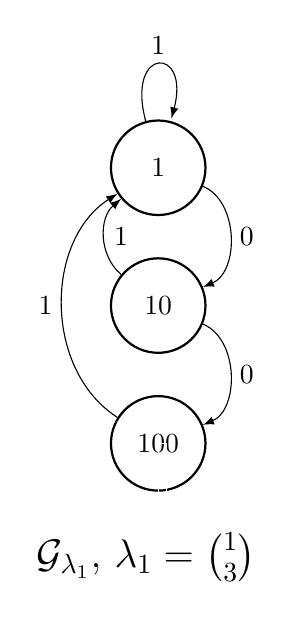
\begin{tikzpicture}[>=latex]
    \node[Dom Node] (a) at (0,0) {$1$};
    \node[Dom Node] (b) at (0,-1.75) {$10$};
    \node[Dom Node] (c) at (0,-3.5) {$100$};
    \draw[->] (a) edge [loop above] node[above] {$1$} (a);
    \draw[->] (a) edge [bend left=67.5] node[right] {$0$} (b);
    \draw[->] (b) edge [bend left=50] node[right] {$1$} (a);
    \draw[->] (b) edge [bend left=67.5] node[right] {$0$} (c);
    \draw[->] (c) edge [bend left=57.5] node[left] {$1$} (a);
    \draw[white] (0,-3.5) rectangle (0.1,-4.5);

    \node[anchor=north] at (current bounding box.south) {\Large $\GG{\lambda_1},\, \lambda_1 = \binom{1}{3}$};
\end{tikzpicture}

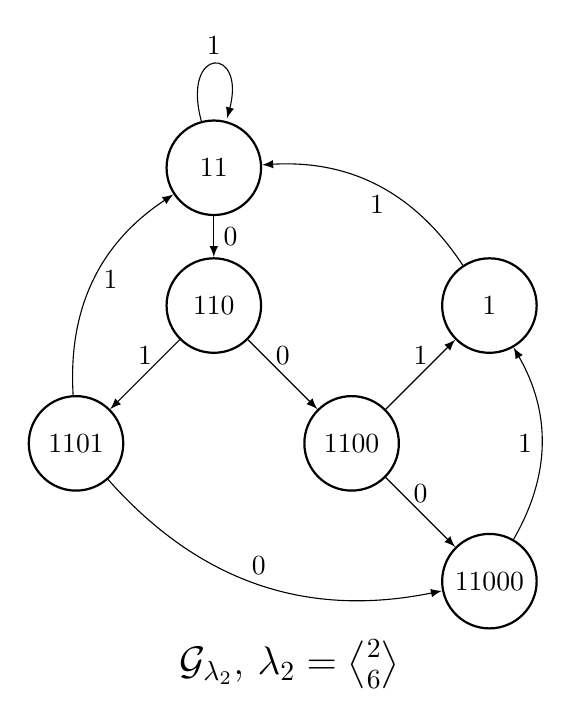
\begin{tikzpicture}[>=latex]
    \node[Dom Node] (a) at (0,0) {$11$};
    \node[Dom Node] (b) at (0,-1.75) {$110$};
    \node[Dom Node] (c) at (-1.75,-3.5) {$1101$};
    \node[Dom Node] (d) at (1.75,-3.5) {$1100$};
    \node[Dom Node] (e) at (3.5,-5.25) {$11000$};
    \node[Dom Node] (f) at (3.5,-1.75) {$1$};

    \draw[->] (a) edge [loop above] node[above] {$1$} (a);
    \draw[->] (a) edge [] node[right] {$0$} (b);
    \draw[->] (b) edge [] node [above] {$1$} (c);
    \draw[->] (b) edge [] node [above] {$0$} (d);
    \draw[->] (c) edge [bend left] node [right] {$1$} (a);
    \draw[->] (c) edge [bend right] node [above] {$0$} (e);
    \draw[->] (d) edge [] node [above] {$0$} (e);
    \draw[->] (d) edge [] node [above] {$1$} (f);
    \draw[->] (e) edge [bend right] node [left] {$1$} (f);
    \draw[->] (f) edge [bend right] node [below] {$1$} (a);

    \node[anchor=north] at (current bounding box.south) {\Large $\GG{\lambda_2},\, \lambda_2 = \genfrac{<}{>}{0pt}{}{2}{6}$};
\end{tikzpicture}

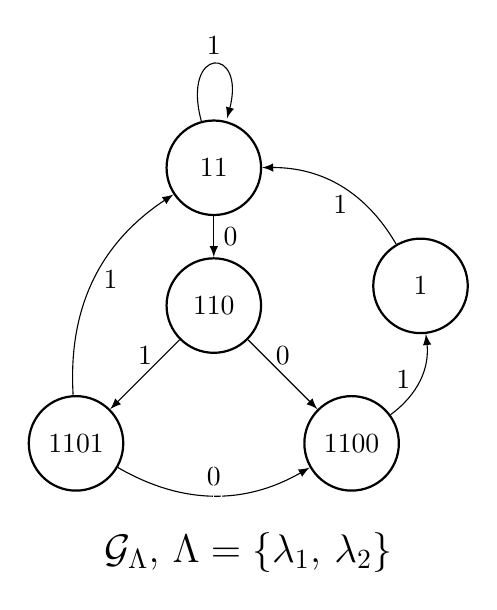
\begin{tikzpicture}[>=latex]
    \node[Dom Node] (a) at (0,0) {$11$};
    \node[Dom Node] (b) at (0,-1.75) {$110$};
    \node[Dom Node] (c) at (-1.75,-3.5) {$1101$};
    \node[Dom Node] (d) at (1.75,-3.5) {$1100$};
    \node[Dom Node] (e) at (2.625,-1.5) {$1$};

    \draw[->] (a) edge [loop above] node[above] {$1$} (a);
    \draw[->] (a) edge [] node[right] {$0$} (b);
    \draw[->] (b) edge [] node [above] {$1$} (c);
    \draw[->] (b) edge [] node [above] {$0$} (d);
    \draw[->] (c) edge [bend left] node [right] {$1$} (a);
    \draw[->] (c) edge [bend right] node [above] {$0$} (d);
    \draw[->] (d) edge [bend right] node [left] {$1$} (e);
    \draw[->] (e) edge [bend right] node [below] {$1$} (a);

    \draw[white] (0,-3.5) rectangle (0.1,-4.5);

    \node[anchor=north] at (current bounding box.south) {\Large $\GG{\Lambda},\, \Lambda = \left\{ \lambda_1,\, \lambda_2 \right\}$};
\end{tikzpicture}
}

    \caption{\fix{Ask Martina to help fix these to be on top of one another} Minimal automata $\GG{\lambda_1}$, $\GG{\lambda_2}$, and $\GG{\Lambda}$ representing respectively $\lambda_1$, $\lambda_2$, and $\Lambda = \{\lambda_1, \lambda_2\}$ from the Example in Section~\ref{sec:tool:example}.}%{ex:tool:set}.}
    \label{fig:dominant-set}
\end{figure*}

\subsection{Scalable automata generation}%
\label{sec:tool:scalability}%

Intuitively, the time required for generating an automaton is directly correlated to its size, i.e., more vertices lead to a larger exploration time and hence to a larger automaton-construction time. 
Additionally, the automata-based representation can be used in embedded devices, e.g., to monitor the satisfaction of a constraint.
Thus, space and memory requirements create a clear need for the automaton to be minimal.

We provide a brief discussion on the minimum number of vertices needed to express the automaton corresponding to the weakly hard constraints presented in Definition~\ref{def:weakly-hard}.
The structure of the minimal automaton depends on the type of constraint.
For example, to describe an \tAH{} constraint $\anyhit{ah}$ we need to keep track of the number and the position of the deadline hits we encountered in the past $k_{ah}$ outcomes, giving us a number of vertices that corresponds to the binomial coefficient \emph{$k_{ah}$ choose $x_{ah}$}.
The \tAM{} constraint can be reduced to the \tAH{} constraint and hence we easily obtain the number of its vertices.
For the \tRM{} constraint, the number of vertices is also obvious, as we need to count the number of consecutive deadlines that have been missed, and return to the initial state as soon as the following outcome is a hit.
Denoting with $\mathrm{s}\left(\lambda\right)$ the function that counts the number of vertices of the minimal automaton corresponding to the constraint $\lambda$, we obtain:
\begin{equation*}
    \begin{aligned}
        \tAH{}:\phantom{\textbf{iii}}\lambda_{ah} = \textstyle\anyhit{ah} & \Rightarrow \mathrm{s}\left(\lambda_{ah}\right) = \frac{k_{ah}!}{x_{ah}!\,(k_{ah}-x_{ah})!}  \\
        \tAM{}:\phantom{\textbf{s}}\lambda_{am} = \textstyle\anymiss{am} & \Rightarrow \mathrm{s}\left(\lambda_{am}\right) = \frac{k_{am}!}{x_{am}!\,(k_{am}-x_{am})!}  \\
        \tRM{}:\phantom{\textbf{s}}\lambda_{rm} = \textstyle\rowmiss{rm} & \Rightarrow \mathrm{s}\left(\lambda_{rm}\right) = x_{rm}+1 \\
    \end{aligned}
\end{equation*}
e.g., the minimal automaton for the \tAM{} constraint $\overbar{\binom{5}{20}}$ includes $15\,504$ vertices.

The \tRH{} constraint, $\rowhit{rh}$ is more interesting.
When $k_{rh} < 2\,x_{rh}$, the constraint reduces to the hardest constraint $\lhard$, hence the automaton has a single vertex.
If $k_{rh} = 2\,x_{rh}$, it is possible to have a single deadline miss, that can only appear before a sequence of $x_{rh}$ has been recorded, hence the corresponding automaton has $x_{rh} + 1$ vertices.
If $k_{rh} = 2\,x_{rh} + 1$, the number of vertices of the automaton are $x_{rh} + 2$ and subsequent values can be found using recursion.
Specifically,
\begin{equation*}
    \begin{aligned}
        & \tRH{}: \, \lambda_{rh} = \textstyle\rowhit{rh} \Rightarrow \mathrm{s}\left(\lambda_{rh}\right) = \\
        & \begin{cases}
            1 & k_{rh} < 2x_{rh} \\
            x_{rh}+1 & k_{rh} = 2x_{rh} \\
            x_{rh}+2 & k_{rh} = 2x_{rh}+1 \\
            2\, \mathrm{s}\,(\textstyle \genfrac{<}{>}{0pt}{}{x_{rh}}{k_{rh}-1} ) - 
                \mathrm{s}\,(\textstyle \genfrac{<}{>}{0pt}{}{x_{rh}}{k_{rh}-2} ) + 1 & 2x_{rh} + 1 < k_{rh} < 3x_{rh} \\
            \mathrm{s}\,(\textstyle \genfrac{<}{>}{0pt}{}{x_{rh}}{k_{rh}-1} ) + x_{rh} &k_{rh} \geq 3x_{rh}. \\
        \end{cases}
    \end{aligned}
\end{equation*}
%
In contrast to the \tAH{} or \tAM{} constraints, the size of the minimal automaton corresponding to the \tRH{} constraint is linear in the window length $k_{rh}$ in stationarity, i.e., when $k_{rh} \geq 3x_{rh}$.
The linearity property also holds for the \tRM{} constraint.
Intuitively, since the size of the minimal automaton is directly correlated to the scalability, \tRH{} and \tRM{} constraints are preferred for large problems.

\subsection{Example}%
\label{sec:tool:example}%
%
We now provide an example to illustrate how the automata differ between constraint types. 
In particular, we focus on \tAH{} and \tRH{} constraints, that have been the subject of our theoretical investigation. 

Given the two weakly-hard constraints $\lambda_1 = \binom{1}{3}$ and $\lambda_2 = \genfrac{<}{>}{0pt}{}{2}{6}$, we apply Theorems~\ref{thm:dom-rowhit-anyhit} and~\ref{thm:dom-anyhit-rowhit} and confirm that there is no partial ordering between the constraints, i.e. $\lambda_1 \npreceq \lambda_2$ and $\lambda_2 \npreceq \lambda_1$.
Following the steps in Algorithm~\ref{alg:tool:automata}, we generate the \emph{minimal} automaton representations of the two constraints, i.e., $\GG{\lambda_1}$ and $\GG{\lambda_2}$.
The automaton representing the constraint set $\Lambda = \left\{ \lambda_1,\, \lambda_2 \right\}$, i.e., $\GG{\Lambda}$, is also generated and subsequently minimised.
The results are shown in Figure~\ref{fig:dominant-set}, where the leftmost, middle, and rightmost automata correspond respectively to $\GG{\lambda_1}$, $\GG{\lambda_2}$, and $\GG{\Lambda}$.
%\end{example}

One of the most important novelties presented in this paper is the possibility to analyse weakly-hard constraint \emph{sets} containing \emph{all} the weakly-hard constraints types from Definition~\ref{def:weakly-hard}. 
Prior work proposed alternative solutions to the automaton generation problem, handling either a specific type of constraint~\cite{Horssen:2016}, or a separate solution for each individual constraint type~\cite{Linsenmayer:2017}.
Our aim is to switch the focus to the applicability and scalability of the constraint representation, and hence substitute \tAH{} and \tAM{} with \tRH{} and \tRM{} whenever possible.
Being able to analyse sets of constraints in a scalable way brings us one step closer to the analysis of real systems, in which window lengths are quite large.
Additionally, for real systems it is often easier to constrain hits (e.g., via execution in a protected environment without interference) rather than the maximum number or the pattern of deadline misses.

\subsection{\tool{} functionality}%
\label{sec:tool:functionality}%
%
\begin{table*}[t]
    \centering
    \caption{Functions offered by \tool{}.}
    \label{tab:tool:functionality}
    {\renewcommand{\arraystretch}{1.4}
    \begin{tabular}{p{0.39\textwidth}p{0.59\textwidth}}
        \hline\hline
        \textbf{Function} & \textbf{Description} \\ \hline \hline
        \texttt{AnyHitConstraint(x, k)}             & Defines a constraint $\lambda = \anyhit{}$ \\ \hline
        \texttt{AnyMissConstraint(x, k)}            & Defines a constraint $\lambda = \anymiss{}$  \\ \hline
        \texttt{RowHitConstraint(x, k)}             & Defines a constraint $\lambda = \rowhit{}$  \\ \hline
        \texttt{RowMissConstraint(x)}               & Defines a constraint $\lambda = \overline{\left<x\right>}$  \\ \hline
        \texttt{is\_satisfied(Lambda, w)}           & Returns \textbf{true} if $w \vdash \Lambda$, i.e., if the word $w$ satisfies all the constraints in $\Lambda$, and \textbf{false} otherwise (note: can be invoked also passing a single constraint $\lambda$ as parameter) \\ \hline
        \texttt{is\_dominant(lambda1, lambda2)}     & Returns \textbf{true} if $\lambda_1 \preceq \lambda_2$ and \textbf{false} otherwise \\ \hline
        \texttt{is\_equivalent(lambda1, lambda2)}   & Returns \textbf{true} if $\lambda_1 \equiv \lambda_2$ and \textbf{false} otherwise \\ \hline
        \texttt{dominant\_set(Lambda)}              & Returns $\Lambda^* \subseteq \Lambda$ \\ \hline
        \texttt{build\_automaton(Lambda)}           & Returns the automaton $\GG{\Lambda}$ (note: can be invoked also passing a single constraint $\lambda$ as parameter) \\ \hline
        \texttt{minimize\_automaton!(G)}            & Returns the minimal representation of $\GG{\Lambda}$ (note: changes $\GG{\Lambda}$) \\ \hline
        \texttt{random\_sequence(G, N)}             & Returns a word $w,\, \abs{w}=N$ obtained through an $N$-step random walk in $\GG{\Lambda}$ \\ \hline
        \texttt{all\_sequences(G, N)}               & Returns the satisfaction set $\sset{N}{\Lambda}$ corresponding to $\GG{\Lambda}$ \\ \hline\hline
    \end{tabular}
    }
\end{table*}

%
The most relevant functions provided by \tool{} are summarised in Table~\ref{tab:tool:functionality}.\footnote{The package includes a README file that guides the user through the setup of the package and provides simple usage examples. The only prerequisite is the Julia interpreter and compiler, available at \url{https://julialang.org}.}
In addition to the automata generation, the toolbox provides functions to compare constraints and obtain answers about their dominance and equivalence, to reduce a set of constraints to their dominant subset, and to generate sequences of arbitrary length satisfying sets of weakly-hard constraints.
We also included a function that generate the satisfaction set $\sset{N}{\Lambda}$ from a graph $\GG{\Lambda}$.
In addition to the functions presented in Table~\ref{tab:tool:functionality}, additional functions are included as syntactic sugar for a better user experience.
 

\section{Experimental evaluation}
\label{sec:experiment} 
We evaluate here the performance of \tool{}.\footnote{All the reported experiments ran on an Intel Xeon E5-2620 v3 @ 2.40GHz CPU with 126GB RAM memory.}
First, we assess the scalability of the automaton generation, comparing \tool{} with the state-of-the-art \toolLinsenmayer{}~\cite{Linsenmayer:2017, Linsenmayer:2021}.
Then, we conduct a sensitivity analysis of \tool{} to determine which parameters affect the execution time for the automata generation in cases that cannot be handled with other tools, e.g., sets of weakly-hard constraints.
We provide results on how the type of constraints, maximum window length, and constraint set cardinality affect the computation time needed to generate the automaton.
Finally, we investigate the average cardinality of the dominant set as a function of the cardinality of a set of constraints.

% HERE FOR PLACING
\begin{figure*}[t]
    \begin{center}
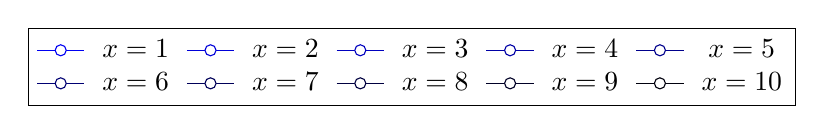
\begin{tikzpicture}
\begin{customlegend}[legend columns=5,legend style={column sep=1ex},legend entries={$x=1$,$x=2$,$x=3$,$x=4$,$x=5$,$x=6$,$x=7$,$x=8$,$x=9$,$x=10$}]
\addlegendimage{blue!95!black, mark=*, mark size=2pt,mark options={fill=white}},
\addlegendimage{blue!85!black, mark=*, mark size=2pt}
\addlegendimage{blue!75!black, mark=*, mark size=2pt}
\addlegendimage{blue!65!black, mark=*, mark size=2pt}
\addlegendimage{blue!55!black, mark=*, mark size=2pt}
\addlegendimage{blue!45!black, mark=*, mark size=2pt}
\addlegendimage{blue!35!black, mark=*, mark size=2pt}
\addlegendimage{blue!25!black, mark=*, mark size=2pt}
\addlegendimage{blue!15!black, mark=*, mark size=2pt}
\addlegendimage{blue! 5!black, mark=*, mark size=2pt}
\end{customlegend}
\end{tikzpicture}
\end{center}

\begin{tikzpicture}
            
    \pgfplotstableread[col sep=comma]{\figdir/data/parsed-julia-any-hit-10-20-mean.csv}{\table}
    \pgfplotstabletranspose{\data}{\table}

    \begin{axis}[% plotting options
	width = 0.265\textwidth,
	height = 0.3\textwidth,
	title style={align=center},
        title = {\tool{}\\\tAH{}\\(baseline $3.7 \mu$s)},
        xlabel = {$i=k-x$},
        ylabel = {$\frac{\text{execution time}}{\text{baseline}}$ (log scale)},
        cycle list name=blue10,   % force me to follow my color list
        xmin=\xstart-1, xmax=\xend, % 1 is to ignore the first data which is the x value
        ymode=log,                % y scale should be logarithmic
        ymin=0.1, ymax=10000,     % may want to change these values
        xtick distance=1,         % we would like to see them all if possible
        % y axes labels, you really want to emphasise the numbers, so no powers of 10
        log ticks with fixed point,
        y tick label style={/pgf/number format/1000 sep = {}},
        % grid to make the graph more readable
        grid=both,
        grid style={black!70, densely dotted},
        minor grid style={black!10, densely dotted},
        ]

        % the actual plot in a foreach
        \pgfplotsforeachungrouped \n in {\xstart,...,\xend}{
            \addplot+ table [x expr=\coordindex-1, y index=\n] {\data};
        }
    \end{axis}
\end{tikzpicture}
%
\hspace{-5mm}
%
\begin{tikzpicture}

    \pgfplotstableread[col sep=comma]{\figdir/data/parsed-matlab-any-hit-10-20-mean.csv}{\table}
    \pgfplotstabletranspose{\data}{\table}

    \begin{axis}[% plotting options
	width = 0.265\textwidth,
	height = 0.3\textwidth,
	title style={align=center},
        title = {\toolLinsenmayer{}~\cite{Linsenmayer:2017}\\\tAH{}\\(baseline $32.4$ms)},
        xlabel = {$i=k-x$},
        %ylabel = {$\frac{\text{execution time}}{\text{baseline}}$ (logarithmic scale)},
        cycle list name=blue10,   % force me to follow my color list
        xmin=\xstart-1, xmax=\xend, % 1 is to ignore the first data which is the x value
        ymode=log,                % y scale should be logarithmic
        ymin=0.1, ymax=10000,     % may want to change these values
        xtick distance=1,         % we would like to see them all if possible
        % y axes labels, you really want to emphasise the numbers, so no powers of 10
        log ticks with fixed point,
        y tick label style={/pgf/number format/1000 sep = {}},
        % grid to make the graph more readable
        grid=both,
        grid style={black!70, densely dotted},
        minor grid style={black!10, densely dotted},
        ]

	\addplot {-1};
        % the actual plot in a foreach
        \pgfplotsforeachungrouped \n in {2,...,\xend}{
            \addplot+ table [x expr=\coordindex-1, y index=\n] {\data};
        }
    \end{axis}
\end{tikzpicture}
%
\hspace{-5mm}
%
\begin{tikzpicture}

    \pgfplotstableread[col sep=comma]{\figdir/data/parsed-julia-row-hit-10-20-mean.csv}{\table}
    \pgfplotstabletranspose{\data}{\table}

    \begin{axis}[% plotting options
	width = 0.265\textwidth,
	height = 0.3\textwidth,
	title style={align=center},
        title = {\tool{}\\\tRH{}\\(baseline $3.2 \mu$s)},
        xlabel = {$i=k-x$},
        %ylabel = {$\frac{\text{execution time}}{\text{baseline}}$ (logarithmic scale)},
        cycle list name=blue10,   % force me to follow my color list
        xmin=\xstart-1, xmax=\xend, % 1 is to ignore the first data which is the x value
        ymode=log,                % y scale should be logarithmic
        ymin=0.1, ymax=10000,     % may want to change these values
        xtick distance=1,         % we would like to see them all if possible
        % y axes labels, you really want to emphasise the numbers, so no powers of 10
        log ticks with fixed point,
        y tick label style={/pgf/number format/1000 sep = {}},
        % grid to make the graph more readable
        grid=both,
        grid style={black!70, densely dotted},
        minor grid style={black!10, densely dotted},
        ]

        % the actual plot in a foreach
        \pgfplotsforeachungrouped \n in {\xstart,...,\xend}{
            \addplot+ table [x expr=\coordindex-1, y index=\n] {\data};
        }
    \end{axis}
\end{tikzpicture}
%
\hspace{-5mm}
%
\begin{tikzpicture}

    \pgfplotstableread[col sep=comma]{\figdir/data/parsed-matlab-row-hit-10-20-mean.csv}{\table}
    \pgfplotstabletranspose{\data}{\table}

    \begin{axis}[% plotting options
	width = 0.265\textwidth,
	height = 0.3\textwidth,
	title style={align=center},
        title = {\toolLinsenmayer{}~\cite{Linsenmayer:2017}\\\tRH{}\\(baseline $17.7$ms)},
        xlabel = {$i=k-x$},
        %ylabel = {$\frac{\text{execution time}}{\text{baseline}}$ (logarithmic scale)},
        cycle list name=blue10,   % force me to follow my color list
        xmin=\xstart-1, xmax=\xend, % 1 is to ignore the first data which is the x value
        ymode=log,                % y scale should be logarithmic
        ymin=0.1, ymax=10000,     % may want to change these values
        xtick distance=1,         % we would like to see them all if possible
        % y axes labels, you really want to emphasise the numbers, so no powers of 10
        log ticks with fixed point,
        y tick label style={/pgf/number format/1000 sep = {}},
        % grid to make the graph more readable
        grid=both,
        grid style={black!70, densely dotted},
        minor grid style={black!10, densely dotted},
        ]

	\addplot {-1};
        % the actual plot in a foreach
        \pgfplotsforeachungrouped \n in {2,...,\xend}{
            \addplot+ table [x expr=\coordindex-1, y index=\n] {\data};
        }
    \end{axis}
\end{tikzpicture}

    \caption{Execution time comparison for \tAH{} and \tRH{} constraints with \tool{} and \toolLinsenmayer{}~\cite{Linsenmayer:2017} increasing the difference between window size and number of hits constrained.
        Baseline values are reported on top of the corresponding plots.}
    \label{fig:timing}
\end{figure*}

\subsection{Comparing \tool{} and \toolLinsenmayer{}}%
\label{sec:comparative_evaluation}%

The literature contribution that is closest to our research is \toolLinsenmayer{}~\cite{Linsenmayer:2017, Linsenmayer:2021}.
\toolLinsenmayer{}'s analysis of weakly-hard tasks is also based on the construction of automata.
While \toolLinsenmayer{} handles only one weakly-hard constraint at a time, it can construct the automaton that correspond to \tAH{} and \tRH{} constraints, making it the reference in terms of analysis capabilities.
\toolLinsenmayer{} is implemented in MATLAB, while \tool{} is implemented in Julia.
Hence, comparing the execution times of the two (on their own) is pointless.
Furthermore, we are more interested in assessing the scalability to an increase in the constraint window size than the absolute numbers for the execution times.
We therefore define a baseline case, for a fair comparison, i.e., the reported results are fractions and multiples of the baseline, which is different for each tool and constraint type.

To test the scalability of the automaton generation, we ask both \tool{} and \toolLinsenmayer{} to generate the automata that correspond to the \tAH{} $\binom{x}{k}$ and \tRH{} $\genfrac{<}{>}{0pt}{}{x}{k}$ constraints for $x \in \{1,2,\dots,10\}$, $k=x+i$ and $i \in \{0,1,\dots,10\}$.
We divide the obtained results by the baseline value, i.e., the execution time needed for the corresponding tool to generate the automaton for the given constraint type, $x=2$ and $k=4$.\footnote{The choice of the baseline case reflects the simplest constraint that is correctly handled by both \tool{} and \toolLinsenmayer{}. Comparing the methods, we unveiled that \toolLinsenmayer{} is unable to find an automaton for constraints in which $x=1$. The two plots for \toolLinsenmayer{} in Figure~\ref{fig:timing} do not contain results for $x=1$ (white filled markers) precisely due to this problem.}

Figure~\ref{fig:timing} shows the mean value of the execution time for the automaton generation, divided by the corresponding baseline value, using a logarithmic y-axis.
The baseline computation times for \tAH{} constraint are $3.7 \mu$s for \tool{} and   $32.4$ms for \toolLinsenmayer{}. On the contrary, for a \tRH{} constraint, the baseline computation time is $3.2 \mu$s for \tool{} and $17.7$ms for \toolLinsenmayer{}.
Due to the extensive computational time necessary to build the automata using \toolLinsenmayer{}, each automaton was built $30$ times (i.e., each point in the figure is the mean of $30$ executions).
\tool{} is significantly faster, thus, each automata was built $100\,000$ times to reduce the execution time variance.

\toolLinsenmayer{} represents a weakly-hard constraint with a slightly different, yet equivalent automaton to the one generated by \tool{}.
In particular, the automaton generated by \toolLinsenmayer{} has fewer vertices and weights on the edges encode the number of consecutive deadline misses allowed between the vertices.
Thus, a transition between two vertices in \toolLinsenmayer{} is not equivalent to one outcome (as for \tool{}), reducing flexibility, i.e., making it harder for example to automatically generate code to monitor the outcomes of task executions.
Multiple successive outcomes for each transition also complicate the handling of sets of weakly-hard constraints.
In terms of scalability, an automaton representation with fewer nodes may sound more efficient.
However, we show that \tool{} scales better than \toolLinsenmayer{} by more than an order of magnitude.
The baseline numbers show that \tool{} is also significantly faster in absolute terms.

Comparing the scalability of the two tools for \tAH{} constraints (leftmost plots), we observe that \tool{} is more than an order of magnitude faster than \toolLinsenmayer{}.
On the contrary, for \tRH{} constraints (rightmost plots), we experience a speedup of almost two orders of magnitude for high values of $i = k - x$.
The scalability of the \tRH{} constraints are further investigated in the following subsection.

\subsection{Evaluating \tRH{} constraints}
\label{sec:rowhit_evaluation}

In the previous subsection we discussed the scalability of \tool{} compared to the state-of-the-art.
Despite improvements of more than an order of magnitude (not considering the baseline), the time necessary to construct the automata for \tAH{} constraints grows rapidly with increasing window lengths.
Motivated by the ongoing discussion on the practical importance of consecutive deadline hits~\cite{Akesson:2020, Vreman:2021} and the scalability considerations presented in Section~\ref{sec:tool:scalability}, we now perform an extensive evaluation of the scalability of the \tRH{} constraints.

\begin{figure}[t]
    \centering
\begin{tikzpicture}
            
    %\pgfplotstableread[col sep=comma]{figs/data/parsed-manipulaed-rowhit-25-100-median.csv}{\data}
    \pgfplotstableread[col sep=comma]{\figdir/data/parsed-rowhit-15-85-mean.csv}{\data}

    \begin{axis}[% plotting options
        width = 0.85\textwidth,
        height = 0.5\textwidth,
        title style={align=center},
        ylabel style={align=center, yshift=-0.6cm},
        xlabel = {$i=k-x$},
        ylabel = {execution time [s]\\(log scale)},
        xmin=0, xmax=85,
        %xmin=0, xmax=75,
        ymode=log,
        ymin=-14, ymax=30,     % may want to change these values
        % y axes labels, you really want to emphasise the numbers, so no powers of 10
        log ticks with fixed point,
        y tick label style={/pgf/number format/1000 sep = {}},
        % grid to make the graph more readable
        grid=both,
        grid style={black!70, densely dotted},
        minor grid style={black!10, densely dotted},
        legend pos=south east]

        \addplot[blue!40,ultra thick,mark=none] table [x index=0, y index=1] {\data}; \addlegendentry{$x=1$}
        \addplot[blue!50,ultra thick,mark=none, forget plot] table [x index=0, y index=2] {\data};
        \addplot[blue!60,ultra thick,mark=none, forget plot] table [x index=0, y index=3] {\data};
        \addplot[blue!70,ultra thick,mark=none, forget plot] table [x index=0, y index=4] {\data};
        \addplot[blue!75,ultra thick,mark=none, forget plot] table [x index=0, y index=5] {\data};
        \addplot[blue!80,ultra thick,mark=none, forget plot] table [x index=0, y index=6] {\data};
        \addplot[blue!85,ultra thick,mark=none, forget plot] table [x index=0, y index=7] {\data};
        \addplot[blue!90,ultra thick,mark=none, forget plot] table [x index=0, y index=8] {\data};
        \addplot[blue!95,ultra thick,mark=none, forget plot] table [x index=0, y index=9] {\data};
        \addplot[blue,ultra thick,mark=none, forget plot] table [x index=0, y index=10] {\data};
        \addplot[black!10!blue,ultra thick,mark=none, forget plot] table [x index=0, y index=11] {\data};
        \addplot[black!20!blue,ultra thick,mark=none, forget plot] table [x index=0, y index=12] {\data};
        \addplot[black!30!blue,ultra thick,mark=none, forget plot] table [x index=0, y index=13] {\data};
        \addplot[black!40!blue,ultra thick,mark=none, forget plot] table [x index=0, y index=14] {\data};
        \addplot[black!50!blue,ultra thick,mark=none] table [x index=0, y index=15] {\data}; \addlegendentry{$x=15$}

    \end{axis}
\end{tikzpicture}

    \caption{Mean execution time of the generation \tRH{} constraint automaton.}
    \label{fig:extensive_rowhit}
\end{figure}

Using \tool{}, we generate the automaton corresponding to the \tRH{} $\genfrac{<}{>}{0pt}{}{x}{k}$ constraints for $x \in \{1,2,\dots,15\}$, $k \in \{x,x+1,\dots,100\}$.
To the best of our knowledge, this is the first research work that generates automata representations of weakly-hard constraints with window lengths above $100$.
Figure~\ref{fig:extensive_rowhit} displays the mean execution time over $100$ executions for the automata generation using a logarithmic scale, showing a piecewise exponential growth of execution time with some jumps.
Despite having constraints with window lengths up to $k=100$, the worst reported execution time is below $7$ seconds; reinforcing the arguments in favour of using \tRH{} rather than \tAH{} constraints.

Another interesting consideration is related to the jumps in the execution time that each line shows when reaching certain values of $x$ and $k$.
This follows from the choice of using integers to represent words in \tool{}.
For constraints where $2x+k \geq 64$, $64$ bit integers are not enough to represent all sequences, and \tool{} consequently converts the sequence representation to big integers (using more than $64$ bits).
This representation requires additional resources (memory and computation), hence producing execution time jumps.

\begin{figure*}[t]
    \begin{tikzpicture}
            
    \pgfplotstableread[col sep=comma]{\figdir/data/parsed-set-NO-2.csv}{\data}

    \begin{axis}[% plotting options
        width = 0.255\textwidth,
        height = 0.3\textwidth,
        title style={align=center},
        ylabel style={align=center},
        title = {$\abs{\Lambda^*}=2$\\Without \tRH{}},
        xlabel = {$k_{\max}$},
        ylabel = {execution time [s]\\(log scale)},
        %cycle list name=blue10,   % force me to follow my color list
        xmin=10, xmax=30,
        ymode=log,                % y scale should be logarithmic
        ymin=0.00001, ymax=1000,     % may want to change these values
        %xtick distance=1,         % we would like to see them all if possible
        % y axes labels, you really want to emphasise the numbers, so no powers of 10
        log ticks with fixed point,
        y tick label style={/pgf/number format/1000 sep = {}},
        % grid to make the graph more readable
        grid=both,
        grid style={black!70, densely dotted},
        minor grid style={black!10, densely dotted}]

        \addplot+[name path=mmax,blue!70,mark=none,smooth] table [x index=0, y index=2] {\data};
        \addplot+[name path=mmin,blue!70,mark=none,smooth] table [x index=0, y index=3] {\data};
        \addplot[blue,opacity=0.3] fill between[of=mmax and mmin];


        \addplot+[blue,thick,mark=*,mark size=1pt] table [x index=0, y index=1] {\data};
    \end{axis}
\end{tikzpicture}
%
\hspace{-5mm}
%
\begin{tikzpicture}
            
    \pgfplotstableread[col sep=comma]{\figdir/data/parsed-set-NO-4.csv}{\data}

    \begin{axis}[% plotting options
        width = 0.255\textwidth,
        height = 0.3\textwidth,
        title style={align=center},
        ylabel style={align=center},
        title = {$\abs{\Lambda^*}=4$\\Without \tRH{}},
        xlabel = {$k_{\max}$},
        %cycle list name=blue10,   % force me to follow my color list
        xmin=10, xmax=30,
        ymode=log,                % y scale should be logarithmic
        ymin=0.00001, ymax=1000,     % may want to change these values
        %xtick distance=1,         % we would like to see them all if possible
        % y axes labels, you really want to emphasise the numbers, so no powers of 10
        log ticks with fixed point,
        y tick label style={/pgf/number format/1000 sep = {}},
        % grid to make the graph more readable
        grid=both,
        grid style={black!70, densely dotted},
        minor grid style={black!10, densely dotted}]

        \addplot+[name path=mmax,blue!70,mark=none,smooth] table [x index=0, y index=2] {\data};
        \addplot+[name path=mmin,blue!70,mark=none,smooth] table [x index=0, y index=3] {\data};
        \addplot[blue,opacity=0.3] fill between[of=mmax and mmin];


        \addplot+[blue,thick,mark=*,mark size=1pt] table [x index=0, y index=1] {\data};
    \end{axis}
\end{tikzpicture}
%
\hspace{-5mm}
%
\begin{tikzpicture}
            
    \pgfplotstableread[col sep=comma]{\figdir/data/parsed-set-RH-2.csv}{\data}

    \begin{axis}[% plotting options
        width = 0.255\textwidth,
        height = 0.3\textwidth,
        title style={align=center},
        ylabel style={align=center},
        title = {$\abs{\Lambda^*}=2$\\With \tRH{}},
        xlabel = {$k_{\max}$},
        %cycle list name=blue10,   % force me to follow my color list
        xmin=10, xmax=30,
        ymode=log,                % y scale should be logarithmic
        ymin=0.00001, ymax=1000,     % may want to change these values
        %xtick distance=1,         % we would like to see them all if possible
        % y axes labels, you really want to emphasise the numbers, so no powers of 10
        log ticks with fixed point,
        y tick label style={/pgf/number format/1000 sep = {}},
        % grid to make the graph more readable
        grid=both,
        grid style={black!70, densely dotted},
        minor grid style={black!10, densely dotted}]

        \addplot+[name path=mmax,blue!70,mark=none,smooth] table [x index=0, y index=2] {\data};
        \addplot+[name path=mmin,blue!70,mark=none,smooth] table [x index=0, y index=3] {\data};
        \addplot[blue,opacity=0.3] fill between[of=mmax and mmin];


        \addplot+[blue,thick,mark=*,mark size=1pt] table [x index=0, y index=1] {\data};
    \end{axis}
\end{tikzpicture}
%
\hspace{-5mm}
%
\begin{tikzpicture}
            
    \pgfplotstableread[col sep=comma]{\figdir/data/parsed-set-RH-4.csv}{\data}

    \begin{axis}[% plotting options
        width = 0.255\textwidth,
        height = 0.3\textwidth,
        title style={align=center},
        ylabel style={align=center},
        title = {$\abs{\Lambda^*}=4$\\With \tRH{}},
        xlabel = {$k_{\max}$},
        %cycle list name=blue10,   % force me to follow my color list
        xmin=10, xmax=30,
        ymode=log,                % y scale should be logarithmic
        ymin=0.00001, ymax=1000,     % may want to change these values
        %xtick distance=1,         % we would like to see them all if possible
        % y axes labels, you really want to emphasise the numbers, so no powers of 10
        log ticks with fixed point,
        y tick label style={/pgf/number format/1000 sep = {}},
        % grid to make the graph more readable
        grid=both,
        grid style={black!70, densely dotted},
        minor grid style={black!10, densely dotted},
        ]

        \addplot+[name path=mmax,blue!70,mark=none,smooth] table [x index=0, y index=2] {\data};
        \addplot+[name path=mmin,blue!70,mark=none,smooth] table [x index=0, y index=3] {\data};
        \addplot[blue,opacity=0.3] fill between[of=mmax and mmin];


        \addplot+[blue,thick,mark=*,mark size=1pt] table [x index=0, y index=1] {\data};
    \end{axis}
\end{tikzpicture}

    \caption{Execution time comparison for the generation of the automaton for sets of constraints with increasing maximum window sizes $\max k$.
        Average values are reported alongside the areas between minimum and maximum execution times.}
    \label{fig:set-comp}
\end{figure*}

\subsection{Analysing sets of weakly-hard constraints}
\label{sec:set_evaluation}

\tool{} is the first tool that provides the ability to analyse sets of weakly-hard constraints.
In the following we conduct a sensitivity analysis to assess the scalability of the automaton generation for a set of weakly hard constraints.
In particular, we are interested in finding how the window size affects the execution time of the tool, and how the composition of the set influences the execution time.

We randomise dominant sets of constraints, imposing that at least one of the constraints has a window size of $k_{\max} \in \left\{ 10,\,11,\,\dots,\,30 \right\}$.
We generate sets with either $\abs{\MDS} = 2$ or $\abs{\MDS} = 4$.
We allow these sets to include one \tRH{} constraint or none.
The results of our study are shown in Figure~\ref{fig:set-comp}.
For each of the values of $k_{\max}$ in the figure, we generate $50$ dominant sets $\MDS$.
The figure shows the average execution time in seconds (as a line) and the area representing the span between minimum and maximum execution time.

The first conclusion that we can draw is that the average execution times follow straight lines in a logarithmic scale, thus clearly pointing to the exponential time complexity inherent to expressive task models, such as the weakly-hard model~\cite{Stigge:2015}.

When the cardinality of the set $\abs{\MDS}$ increases (i.e., comparing the two leftmost and the two rightmost plots) the maximum execution time does not change significantly.
In fact, states that would have been reachable with fewer constraint become unreachable due to the additional constraints pruning the state-space.
However, we experience a slight reduction in the execution time's variance, which follows from the nature of the dominant set.
Comparing two dominant sets, $\MDS_1$ and $\MDS_2$, with the same $k_{\max}$: when $\abs{\MDS_1}=2$ and $\abs{\MDS_2}=4$, the set $\MDS_2$ must include less restrictive constraints (otherwise they would dominate the other constraints in the set).
Hence, the set $\MDS_2$ is less likely to be trivial to analyse.

Finally, including a \tRH{} constraint in the set $\MDS$ increases the execution time by an order of magnitude.
This follows from the complex interconnections between the \tRH{} and remaining weakly-hard constraints.
Particularly, for the \tAH{}, \tAM{}, and \tRM{} constraints it is sufficient to count the deadline hits of the jobs currently in the window; however, the \tRH{} constraints need to keep additional track of when they appeared.
This is further reinforced by the fact that when a dominant set includes a \tRH{} constraint, the other constraints in the set have to be very conservative in order to neither dominate nor be dominated by it.
However, we remark that \tool{} is able to generate an automaton for a set $\MDS$ of $4$ constraints with $k_{\max}=30$, including a \tRH{} constraint, in less than $200$ seconds.

\begin{figure}[t]
    \centering
    \begin{tikzpicture}
            
    \pgfplotstableread[col sep=comma]{\figdir/data/parsed-dominant-set-2-100.csv}{\data}

    \begin{axis}[% plotting options
        width = 0.85\textwidth,
        height = 0.5\textwidth,
        title style={align=center},
        ylabel style={align=center},
        xlabel = {$\abs{\Lambda}$},
        ylabel = {$\abs{\MDS}$},
        ylabel near ticks,
        xlabel near ticks,
        %cycle list name=blue10,   % force me to follow my color list
        xmin=1, xmax=100,
        ymin=1, ymax=12.3,     % may want to change these values
        ytick = {1, 3, 5, 7, 9, 11},
        % y axes labels, you really want to emphasise the numbers, so no powers of 10
        log ticks with fixed point,
        y tick label style={/pgf/number format/1000 sep = {}},
        % grid to make the graph more readable
        grid=both,
        grid style={black!70, densely dotted},
        minor grid style={black!10, densely dotted}]

        \addplot+[name path=mmax,blue!70,mark=none] table [x index=0, y index=2] {\data};
        \addplot+[name path=mmin,blue!70,mark=none] table [x index=0, y index=3] {\data};
        \addplot[blue,opacity=0.3] fill between[of=mmax and mmin];


        \addplot+[blue,ultra thick,mark=none] table [x index=0, y index=1] {\data};
    \end{axis}
\end{tikzpicture}

    \caption{Average cardinality of the dominant set $\MDS$ as a function of $\abs{\Lambda}$ with $k_{\max} = 100$ for $1000$ randomly generated constraint sets $\Lambda$.}
    \label{fig:dominant-set-comparison}
\end{figure}

\subsection{Determining the dominant constraint set}
\label{sec:set_dominant_cardinality}%

In Section~\ref{sec:set_evaluation} we investigated dominant sets $\MDS$ with cardinality $\abs{\MDS} \in \{2,4\}$.
Here we justify why this is a relevant benchmark despite the low cardinality.

We select a maximum window size $k_{\max} = 100$.
The window size is large enough that we can find an expressive variety of constraints without partial ordering.
We randomly generate sets $\Lambda$ containing $\abs{\Lambda} \in \{1,\dots,100\}$ constraints.
For each value of $\abs{\Lambda}$ we generate $1000$ different sets, excluding all the trivial constraints that would reduce to $\lhard$ and $\lweak$.
We then compute the dominant set $\MDS$ corresponding to each set.
Figure~\ref{fig:dominant-set-comparison} shows the average cardinality of $\MDS$ (solid line) and the experienced range (area).

As can be seen, most constraint sets reduce to dominant sets with cardinality less than $4$, thus motivating our investigation of the automaton generation execution time.
Generally, it is also interesting that additional constraints tends to reduce the cardinality of $\MDS$, after a peak is reached.
This is however not surprising seeing as adding constraints increases the chances of the added constraints being dominant over some of the constraints in the set.


\section{Conclusion}
\label{sec:conclusion}
There exists a common misconception that analysing a control system's robustness to packet losses on the network is equivalent to having the control algorithm overrun its timing budget, and vice versa.
This paper proposes an approach to analyse real-time control systems and their stability properties when subject to multiple types of faults.
In particular, we analyse \emph{simultaneous} packet losses on the IO communication channels and computational overruns of the task executing the control algorithm, making the analysis more comprehensive than the state-of-the-art alternatives.

%There exists a common misconception that analysing the control-system's robustness to packet losses on the network is equivalent to having the control algorithm overrun its timing budget, and vice versa.
%The paper primarily proposes two contributions:
%\begin{enumerate*}[label=(\roman*)]
%    \item a method for analysing the stability of embedded control-systems subject to IO packet loss, control computational overruns, and combinations thereof, and
%    \item a comprehensive experimental campaign, highlighting the effects the different fault types have on the system.
%\end{enumerate*}

We envision that the analysis method and the corresponding experimental campaign will be used to improve future analysis methods and correct any misconceptions about how faults interact in computer-controlled systems.
Finally, the paper brings the control analysis closer to the state-of-practice compared to the research literature, because it relies on a probabilistic failure model.
In industrial setups, it is in fact easier to get estimates of the probability of certain events from testing campaigns, rather than to extract complex (but deterministic) guarantees like the validity of a weakly-hard constraint.


\balance
\bibliographystyle{abbrv}
\bibliography{main.bib}

\end{document}
